\documentclass[10pt]{article}
\usepackage{float}
\usepackage{amsmath}
\usepackage{paralist}
\usepackage{setspace}
\usepackage{listings}
\usepackage{graphicx}
\usepackage[english]{babel}
\usepackage{geometry}
\usepackage{subcaption}
\usepackage[utf8]{inputenc}
\usepackage{listings}
\usepackage{color}
\usepackage{subcaption}
\usepackage{hyperref}
\usepackage{eurosym}



\begin{document}


\definecolor{mygreen}{rgb}{0,0.6,0}
\definecolor{mygray}{rgb}{0.5,0.5,0.5}
\definecolor{mymauve}{rgb}{0.58,0,0.82}

\lstset{ %
  backgroundcolor=\color{white},   % choose the background color; you must add \usepackage{color} or \usepackage{xcolor}
  basicstyle=\footnotesize,        % the size of the fonts that are used for the code
  breakatwhitespace=false,         % sets if automatic breaks should only happen at whitespace
  breaklines=true,                 % sets automatic line breaking
  captionpos=b,                    % sets the caption-position to bottom
  commentstyle=\color{mygreen},    % comment style
  deletekeywords={...},            % if you want to delete keywords from the given language
  escapeinside={\%*}{*)},          % if you want to add LaTeX within your code
  extendedchars=true,              % lets you use non-ASCII characters; for 8-bits encodings only, does not work with UTF-8
  frame=tb,	                   % adds a frame around the code
  keepspaces=true,                 % keeps spaces in text, useful for keeping indentation of code (possibly needs columns=flexible)
  keywordstyle=\color{blue},       % keyword style
  language=Octave,                 % the language of the code
  otherkeywords={*,...},           % if you want to add more keywords to the set
  numbers=left,                    % where to put the line-numbers; possible values are (none, left, right)
  numbersep=5pt,                   % how far the line-numbers are from the code
  numberstyle=\tiny\color{mygray}, % the style that is used for the line-numbers
  rulecolor=\color{black},         % if not set, the frame-color may be changed on line-breaks within not-black text (e.g. comments (green here))
  showspaces=false,                % show spaces everywhere adding particular underscores; it overrides 'showstringspaces'
  showstringspaces=false,          % underline spaces within strings only
  showtabs=false,                  % show tabs within strings adding particular underscores
  stepnumber=2,                    % the step between two line-numbers. If it's 1, each line will be numbered
  stringstyle=\color{mymauve},     % string literal style
  tabsize=2,	                   % sets default tabsize to 2 spaces
  title=\lstname                   % show the filename of files included with \lstinputlisting; also try caption instead of title
}

\onehalfspacing
\begin{titlepage}
\begin{center}
% Oberer Teil der Titelseite:


\textsc{\LARGE University of Oldenburg}\\[1.5cm]

\textsc{\Large Computerorientierte Physik}\\[0.5cm]


% Title
\newcommand{\HRule}{\rule{\linewidth}{0.5mm}}
\HRule \\[0.4cm]
{ \huge \bfseries Verteilung ver kürzesten Pfade in skalenfreien Graphen}\\[0.4cm]

\HRule \\[1.5cm]

% Author and supervisor
\begin{minipage}{0.4\textwidth}
\begin{flushleft} \large
\emph{Author:}\\
Jan \textsc{K\"amper}\\
Florian \textsc{B\"orgel}
\end{flushleft}
\end{minipage}
\hfill
\begin{minipage}{0.4\textwidth}
\begin{flushright} \large
\emph{Supervisor:} \\
Alexander \textsc{Hartmann}
\end{flushright}
\end{minipage}
\\[3cm]
\vfill



% Unterer Teil der Seite
{\large \today}

\end{center}

\end{titlepage}
\tableofcontents
\newpage
\listoffigures
\newpage
\listoftables
\newpage

\section{Introduction}
This reports guides through the process of Design of Wind Energy Systems. The different phases are structured in so called CIPs. In the first CIP the main parameters of the turbine to be designed will be fixed and site conditions defined. Then in the second CIP the geometry of the blade will be computed according to Schmitz' and Betz' models. Performance curves are the subject of the third tutorial. CIP 4 treats the tower design. Impact of wakes and wind fields are investigated in CIP 5 before in the last CIP a fatigue load analysis (CIP 6a) and an extreme load analysis (CIP 6b) are carried out.
During this project we have used a set of different tools and programming languages, among those: Matlab, Python, WT-Perf, Fast and Turbsim.

\section{CIP 1: Selection of main parameters and rotor design}
In CIP 1 we were asked to estimate the main parameters of our wind turbine model. In addition we also calculated the airfoil aerodynamics properties and defined the geometry of our blade.
The following table shows the site specific conditions and the limitations for the design process of the wind turbine.\\

\begin{table}[H]
\begin{tabular}{l l l}
\hline
Name & unit & value\\
\hline
Airfoil profile set number	&-&	4\\
Design wind regime	&-&	Rayleigh\\
Target wind regime	&-&	High\\
Weibull A-factor (local)&	m/s&	9\\
Weibull k-factor (local)	&-&	2\\
Rated electrical power	&kW&	3500\\
Number of blades	&-&	3\\
Cut-in wind speed	&m/s&	3.5\\
Cut-out wind speed	&m/s&	25\\
Max. tip speed	&m/s&	82\\
Max. hub height – reference (*)&	m&	100\\
Max. blade length  - reference (*)	&m&	60\\
Blade root length	&m&	5\\
Transmission	&-&	90\\
\hline

\end{tabular}
\label{designparameters}
\caption{Design parameters}
\end{table}
\subsection{Total conversion efficiency}
The total conversion efficiency is used to calculate the amount of energy which can be extracted from the wind flow. Therefore it contains all loses due to mechanical and electrical conversions as the corresponding $c_p$ reference value. The $c_p$ variable describes the maximum amount of energy which can be theoretical extracted from the wind.
Taking all these losses into account we have the following equation for the total conversion efficiency:

\begin{equation}
\text{total conversion efficiency} = c_p * \nu_{el} * nu_{mech} = 	0.4705
\end{equation}

\subsection{Wind Power for nominal electrical power}
The rated electrical power of the wind turbine is 3.500 kW. With the total conversion efficiency we computed in the last section we are now able to estimate how much wind power is needed to obtain nominal electrical power.

\begin{equation}
\text{total wind power} = \frac{\text{nominal power}}{\text{total conversion efficency}} = \frac{3500 kW}{0.4705} = 7439.26 kW
\end{equation}

\subsection{Rated wind speed}
At rated wind speed the turbine is able to extract nominal wind speed. The following equation is used to calculate the power output of the wind turbine. It should be noted that resulting value had to be rounded up. 

\begin{equation}
P_{rated} = 0.5 \cdot c_{total} \cdot \rho \cdot \pi \cdot R^2 \cdot V_{rated}^3
\end{equation}

\begin{tabular}{l l}
where:&\\
$P_{rated}$ &= rated electrical power\\
$c_{total}$ &= total conversion efficiency\\
$\rho$ &= density\\
$R$ &= reference max. blade length\\
$V_{rated}$& = rated wind speed\\
\end{tabular}

This equation can be solved for $V_{rated}$:
\begin{equation}
V_{rated} = \sqrt[3]{\frac{2 \cdot P_{rated}}{\rho\cdot c_{total}\cdot R^2 \cdot \pi}} = 11 m/s
\end{equation}
\subsection{Rotor radius}
To calculate the rotor radius we used equation (3). Instead of solving for $V_{rated}$ we solved for the blade radius.
\begin{equation}
R = \sqrt{\frac{2 \cdot P_{rated}}{c_{total} \cdot \rho \cdot \pi \cdot V_{rated}^3}} = 54 m
\end{equation}
With a hub diameter of 2.5 meters we end up with a blade length of 52.75 m.
\subsection{Rotor area and specific rating}
The rotor area is simply the area which is covered by the rotating blades. That leaves us with:
\begin{equation}
A_{area} = \pi * R^2 = 9161 m^2
\end{equation}
Next we were asked to calculate the specific rating which is defined as:
\begin{equation}
rating = \frac{\text{electrical power}}{area}
\end{equation}
We receive 382.06 W/$m^2$ as specific rating.
\subsection{Rotor rated speed \& design tip speed ratio}
The design tip speed ratio is the ratio between maximum tip speed and rated wind speed of the turbine. The maximum tip speed for the wind turbine is $82 m/s$ and the calculated rated wind speed is $11 m/s$. That leads to a design tip speed ratio $\lambda_d$ of \textbf{7.45}.\\\subsection{Annual Energy Production}
Next, we calculated the rotor rated speed. The rotor rated speed in rotations per minute (rpm) is given by:

\begin{equation}
n = \frac{60s/min \cdot\ \text{max. tip speed}}{2\cdot\pi\cdot R} = 14.5 rpm
\end{equation}
%\subsection{Annual Energy Production}
\subsection{Main aerodynamic properties}
In order to estimate the design lift coefficient, the angle of attack and the drag coefficient we were given an excel sheet with the rotor design profile data for NACA-64-415 and NACA-64-421.
Each sheet consists of 4 columns: angle of attack, lift coefficient, drag coefficient and thrust coefficient. According to the lecture, the optimal lift coefficient is defined as the maximum of the lift-to-drag ratio. Figure~\ref{fig:comparison_lift_to_drag} shows the lift-to-drag ratio for different angles of attack (AOA).

\begin{figure}[htb!]
\begin{subfigure}{0.5\textwidth}
  \centering
  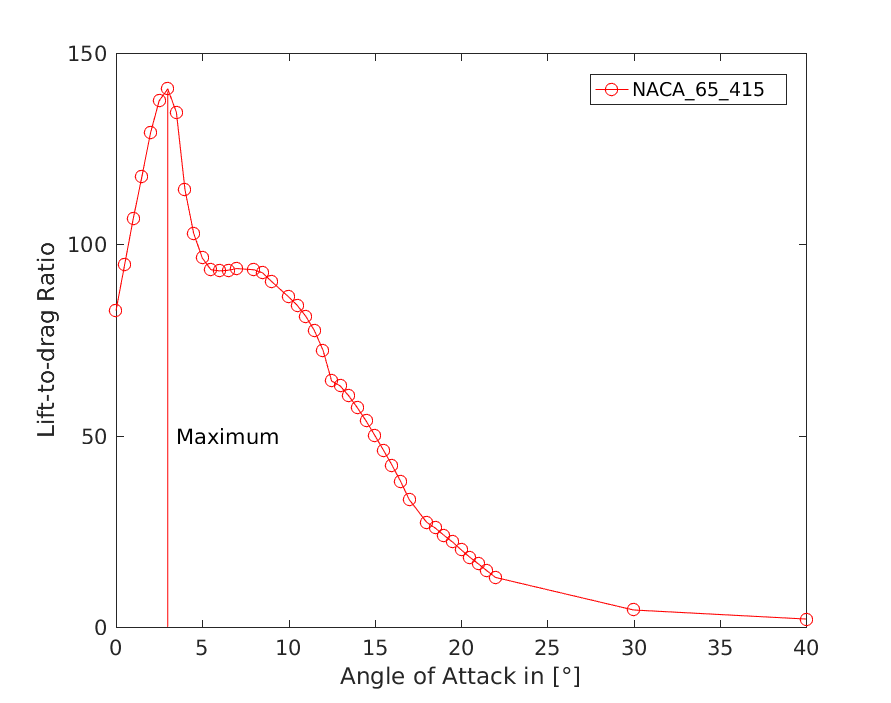
\includegraphics[width=1\linewidth]{../CIP_1/lift_to_drag_ratio_415.png}
  \caption{Lift-to-drag ratio for NACA 65-415}
\end{subfigure}
\begin{subfigure}{0.5\textwidth}
  \centering
  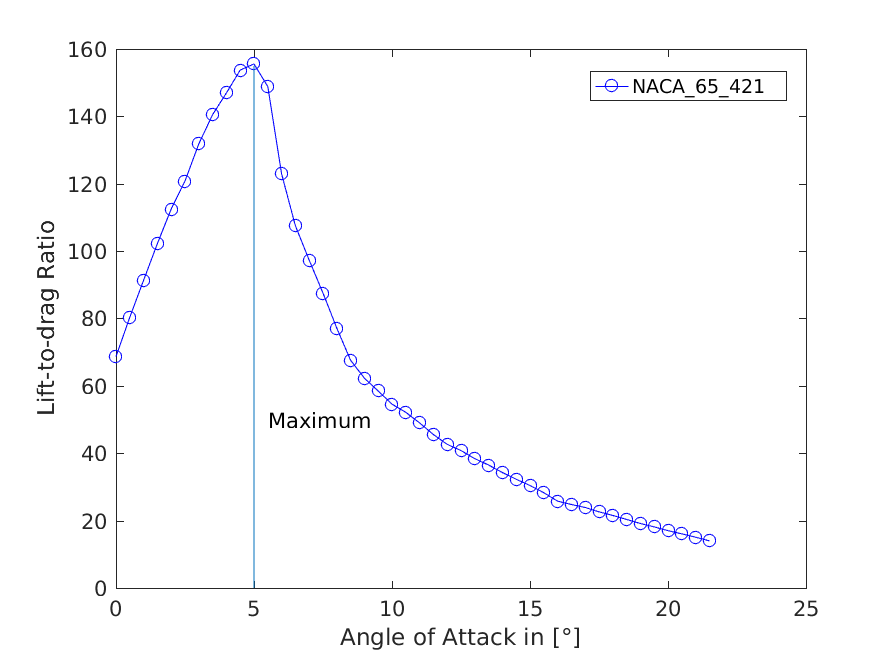
\includegraphics[width=1\linewidth]{../CIP_1/lift_to_drag_ratio_421.png}
  \caption{Lift-to-drag ratio for NACA 65-421}
\end{subfigure}
\caption{Lift-to-drag ratio for different angle of attacks}
\label{fig:comparison_lift_to_drag}
\end{figure}

The figures show that the highest lift-to-drag ratio occurs at low angles of attack. We identified the maximum at 3.0$^\circ$ for NACA 65-415 and 5.0$^\circ$. For higher angles of attack the lift-to-drag ratio shrinks. However in practice there is another method to calculate the optimal design lift coefficient. In the further design we defined the design lift coefficient according to the following equation.
\begin{equation}
c_{l_{design}} = max(cl(max[\frac{c_l}{c_d}], 0.8\cdot c_{l_{max}})
\end{equation}
The results are summarized in the following table:\\
\begin{table}[H]
\begin{tabular}{l | r r r r}
NACA 65-415 & $\alpha$ &$c_l$ &$c_d$ & $c_m$\\
\hline
80\% method& 10 & 1.345 & 0.016 & 0.071\\
lift-to-drag method & 3.0 & 0.710 & 0.005 &  0.088\\
\hline
NACA 65-421 & $\alpha$ &$c_l$ &$c_d$ & $c_m$\\
\hline
80\% method& 11 & 1.255 & 0.026 & 0.055\\
lift-to-drag method & 5.0 & 0.952 & 0.006 &  0.092\\
\end{tabular}
\caption{Main aerodynamic parameters}
\end{table}

As the 80\% method results in a higher lift coefficients for both profiles we selected the corresponding parameters according to the 80\% method.
\newpage
\subsection{Annual Energy Production}
The annual energy production is defined as 
\begin{equation}
\text{total energy production} = \sum n_v \cdot p_v
\end{equation}
with\\
n = number of hours \\
p = power curve\\
v = wind speed\\

With an assumed Rayleigh distribution figure~\ref{fig:ws} was calculated to show the wind speed distribution over a year.

\begin{figure}[H]
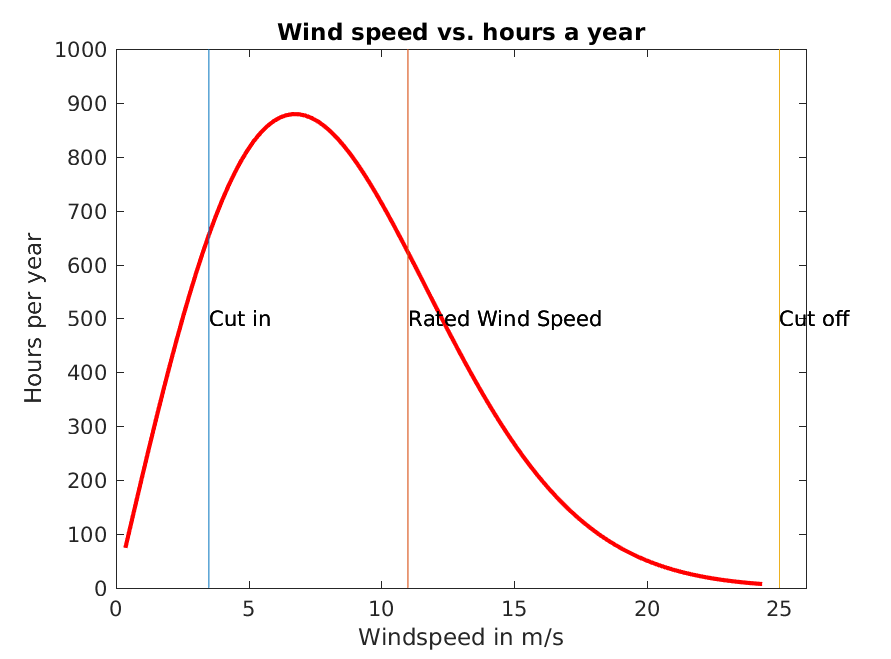
\includegraphics[width=1\linewidth]{../CIP_1/ws_plot.png}
\caption{Wind speed vs. hours per year}
\label{fig:ws}
\end{figure}
In order to proceed with the calculation of the annual energy production the power curve was also calculated, which is shown in the following figure.

\begin{figure}[H]
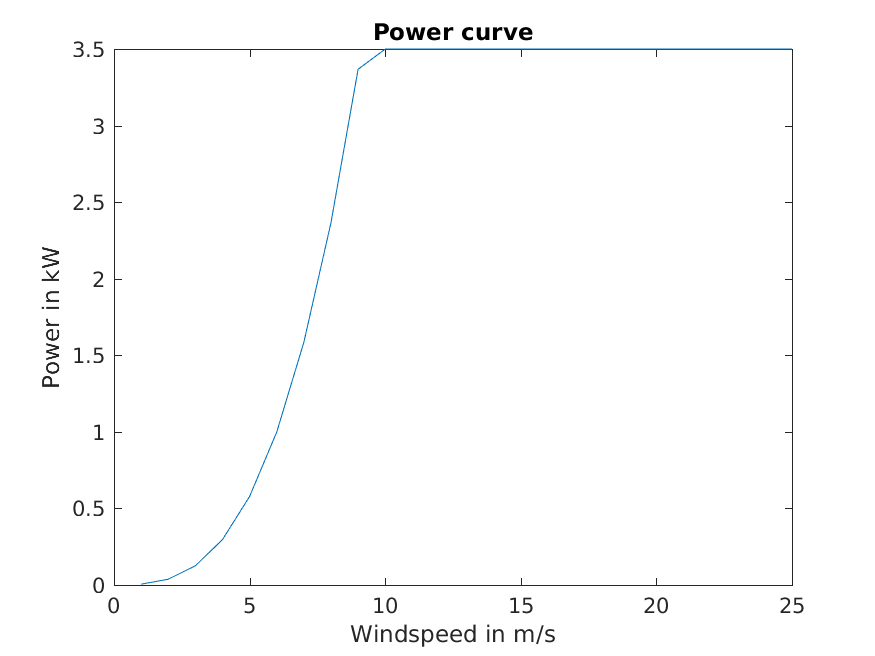
\includegraphics[width=1\linewidth]{../CIP_1/power_curve.png}
\caption{Power curve}
\label{fig:power}
\end{figure}

With these two parameters we were able to calculate the annual energy production which can be extracted by integrating over the whole domain. Figure~\ref{fig:yield} shows the outcome. The annual energy yield is estimated at 18.325 kWh. In order to achieve the highest energy output it is necessary to guarantee a high availability of the turbine. 

\begin{figure}[H]
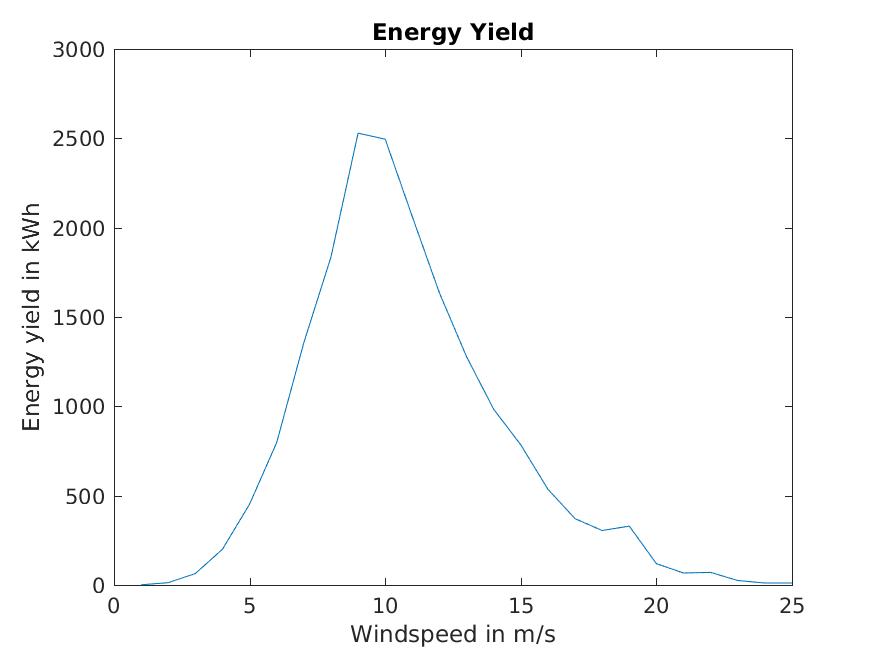
\includegraphics[width=1\linewidth]{../CIP_1/energy_yield.png}
\caption{Annual Energy yield}
\label{fig:yield}
\end{figure}

\section{CIP 2: Advanced BEM }
In the first part of CIP 2 we designed the blade of the wind turbine. In the lecture we discussed two theories which are used to design the blade geometry. Betz and Schmitz theory both have different approaches to calculate the chord length and the twist angle. For the following steps it is import to keep in mind that the given blade consists of 10 blade elements, which are shown in the following figure.
\begin{figure}[H]
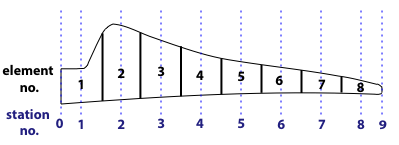
\includegraphics[width=1\linewidth]{../CIP_2/Figures/blade_elements.png}
\caption{Blade Elements}
\label{fig:blade_elemets}
\end{figure}

\subsection{Design your blade according to Betz theory}
Betz theory estimates that the maximum of power that can be extracted from the wind is:
\begin{equation}
P_{betz} = \frac{16}{27}*P_{wind}
\end{equation}
To understand why there is a certain limit, consider that if all energy coming from the wind movement through the turbine the speed afterwards would drop to zero then no new wind could get in and theenergy thus limited.
The principle of Betz's law is derived from the principles of conservation of mass and momentum of the air stream following through and idealized 'actuator disk'.
If we want to design the blade geometry according to this law, the power from the blade element theory has to equal $P_{Betz}$. This leads to the following equations which have been used for the further calculation.\\

Planform:
\begin{equation}
t(r) = 2\pi R \frac{1}{N}\frac{1}{\lambda_a\sqrt{(\lambda_a\frac{r}{R})^2+\frac{4}{9}}}
\end{equation}

Twist angle:
\begin{equation}
\alpha(r) = \arctan(\frac{2}{3}\frac{R}{r\lambda_a)}
\end{equation}
\begin{equation}
\alpha_{twist} = \alpha(r) - \alpha_a
\end{equation}
Using the parameters from CIP 1, we calculated the chord length and the twist angle for each blade segment. An overview is shown in table~\ref{blade_design_betz}.
\begin{table}[H]
\begin{tabular}{c| l l l l l l l l l}
\hline
Station number & 	1&	2&	3	&4	&5	&6	&7	&8	&9\\
\hline
Dist.(rotor center)	m&	4.547&	11.141&	17.734&	24.328&	30.922&	37.516&	44.109&	50.703&	54.000\\
Dist.(blade root)	m&	3.297&	9.891&	16.484&	23.078&	29.672&	36.266&	42.859&	49.453&	52.750\\
\hline
NACA 65-415\\
\hline
Chord length	m&		10.963&	5.989&	3.957&	2.932	&2.324&	1.923&	1.639&	1.428&	1.342\\
Twist angle	deg	&	36.725	&13.436&	5.233&	1.228&	-1.123&	-2.665&	-3.752	&-4.559&	-4.890\\
\hline
NACA 65-421\\
\hline
Chord length	m	&	11.749&	6.418	&4.240&	3.142&	2.490&	2.061	&1.757&	1.531&	1.438
\\
Twist angle	deg	&	35.725&	12.436&	4.233&	0.228	&-2.123&	-3.665	&-4.752&	-5.559	&-5.890\\
\hline
\end{tabular}
\caption{Blade design according to Betz theory}
\label{blade_design_betz}
\end{table}
\subsection{Design according to Schmitz}
The blade design according to Schmitz uses the following equations:\\
Planform:
\begin{equation}
t(r) = \frac{16\pi r}{N c_l}\sin^2(\frac{1}{3}\alpha_1)
\end{equation}

Twist angle:
\begin{equation}
\alpha(r) = \frac{2}{3}\alpha_1
\end{equation}
\begin{equation}
\alpha_{twist} = \alpha(r) - \alpha_a
\end{equation}

where
\begin{equation}
\alpha_1 = \arctan(\frac{R}{\lambda_a rb})
\end{equation}

Using the same approach of the previous section we end up with the following results, shown in table~\ref{blade_design_schmitz}.
\begin{table}[H]
\begin{tabular}{c| l l l l l l l l l}
\hline
Station number & 	1&	2&	3	&4	&5	&6	&7	&8	&9\\
\hline
Dist.(rotor center)	m&	4.547&	11.141&	17.734&	24.328&	30.922&	37.516&	44.109&	50.703&	54.000\\
Dist.(blade root)	m&	3.297&	9.891&	16.484&	23.078&	29.672&	36.266&	42.859&	49.453&	52.750\\
\hline
NACA 65-415\\
\hline
Chord length	m&		6.184 & 5.063 &	3.671&	2.812 & 2.262 & 1.887 & 1.616 &	1.412&	1.328\\
Twist angle	deg	&	28.589	& 12.022 &	4.812 &	1.054 &	-1.210 &	-2.714 &	-3.783	& -4.579 &	-4.906\\
\hline
NACA 65-421\\
\hline
Chord length	m	&	6.628&	5.426&	3.934&	3.013&	2.424&	2.022	&1.732&	1.514&	1.424\\
Twist angle	deg	&	27.589&	11.022&	3.812&	0.0548	&-2.210&	-3.714&-4.783&	-5.579	&-5.906\\
\hline
\end{tabular}
\caption{Blade design according to Schmitz theory}
\label{blade_design_schmitz}
\end{table}
The final blade is designed according to Schmitz theory by a combination of profile 1 and profile 2. The first station has got a cylindrical shape. For stations 2-5 the thinner profile is used, for stations 6-8 the thicker profile is used.Table~\ref{final_blade_design_schmitz} gives more detail about the design rotor blade.
\begin{table}[H]
\begin{tabular}{c| l l l l l l l l l}
\hline
Station number & 	1&	2&	3	&4	&5	&6	&7	&8	&9\\
&Cylinder&65-421&65-421&65-421&65-421& 65-415& 65-415& 65-415&65-415\\
\hline
Blade	m&	3.297&	9.891&	16.484&	23.078&	29.672&	36.266&	42.859&	49.453&	52.750\\
\hline
Chord length	m&	6,628	&5,426&	3,935	&3,014&	2,425&	1,887&	1,617&	1,413&	1,329\\
Twist angle	deg	&	27,590&	11,022&	3,813&	0,055&	-2,211&	-2,715&	-3,783&	-4,580&	-4,907\\
\hline
\end{tabular}
\caption{Final blade design according to Schmitz}
\label{final_blade_design_schmitz}
\end{table}

\subsection{Corrections to BEM}
For the further evaluation of the designed blade we used the blade element momentum theory (BEM). BEM helps to estimate the local forces acting on a wind turbine blade. The first assumption of this theory is the actuator disk model, where we consider a wind turbine in a stream tube, as shown in figure~\ref{fig:actuatordisk}.
\begin{figure}[H]
\centering
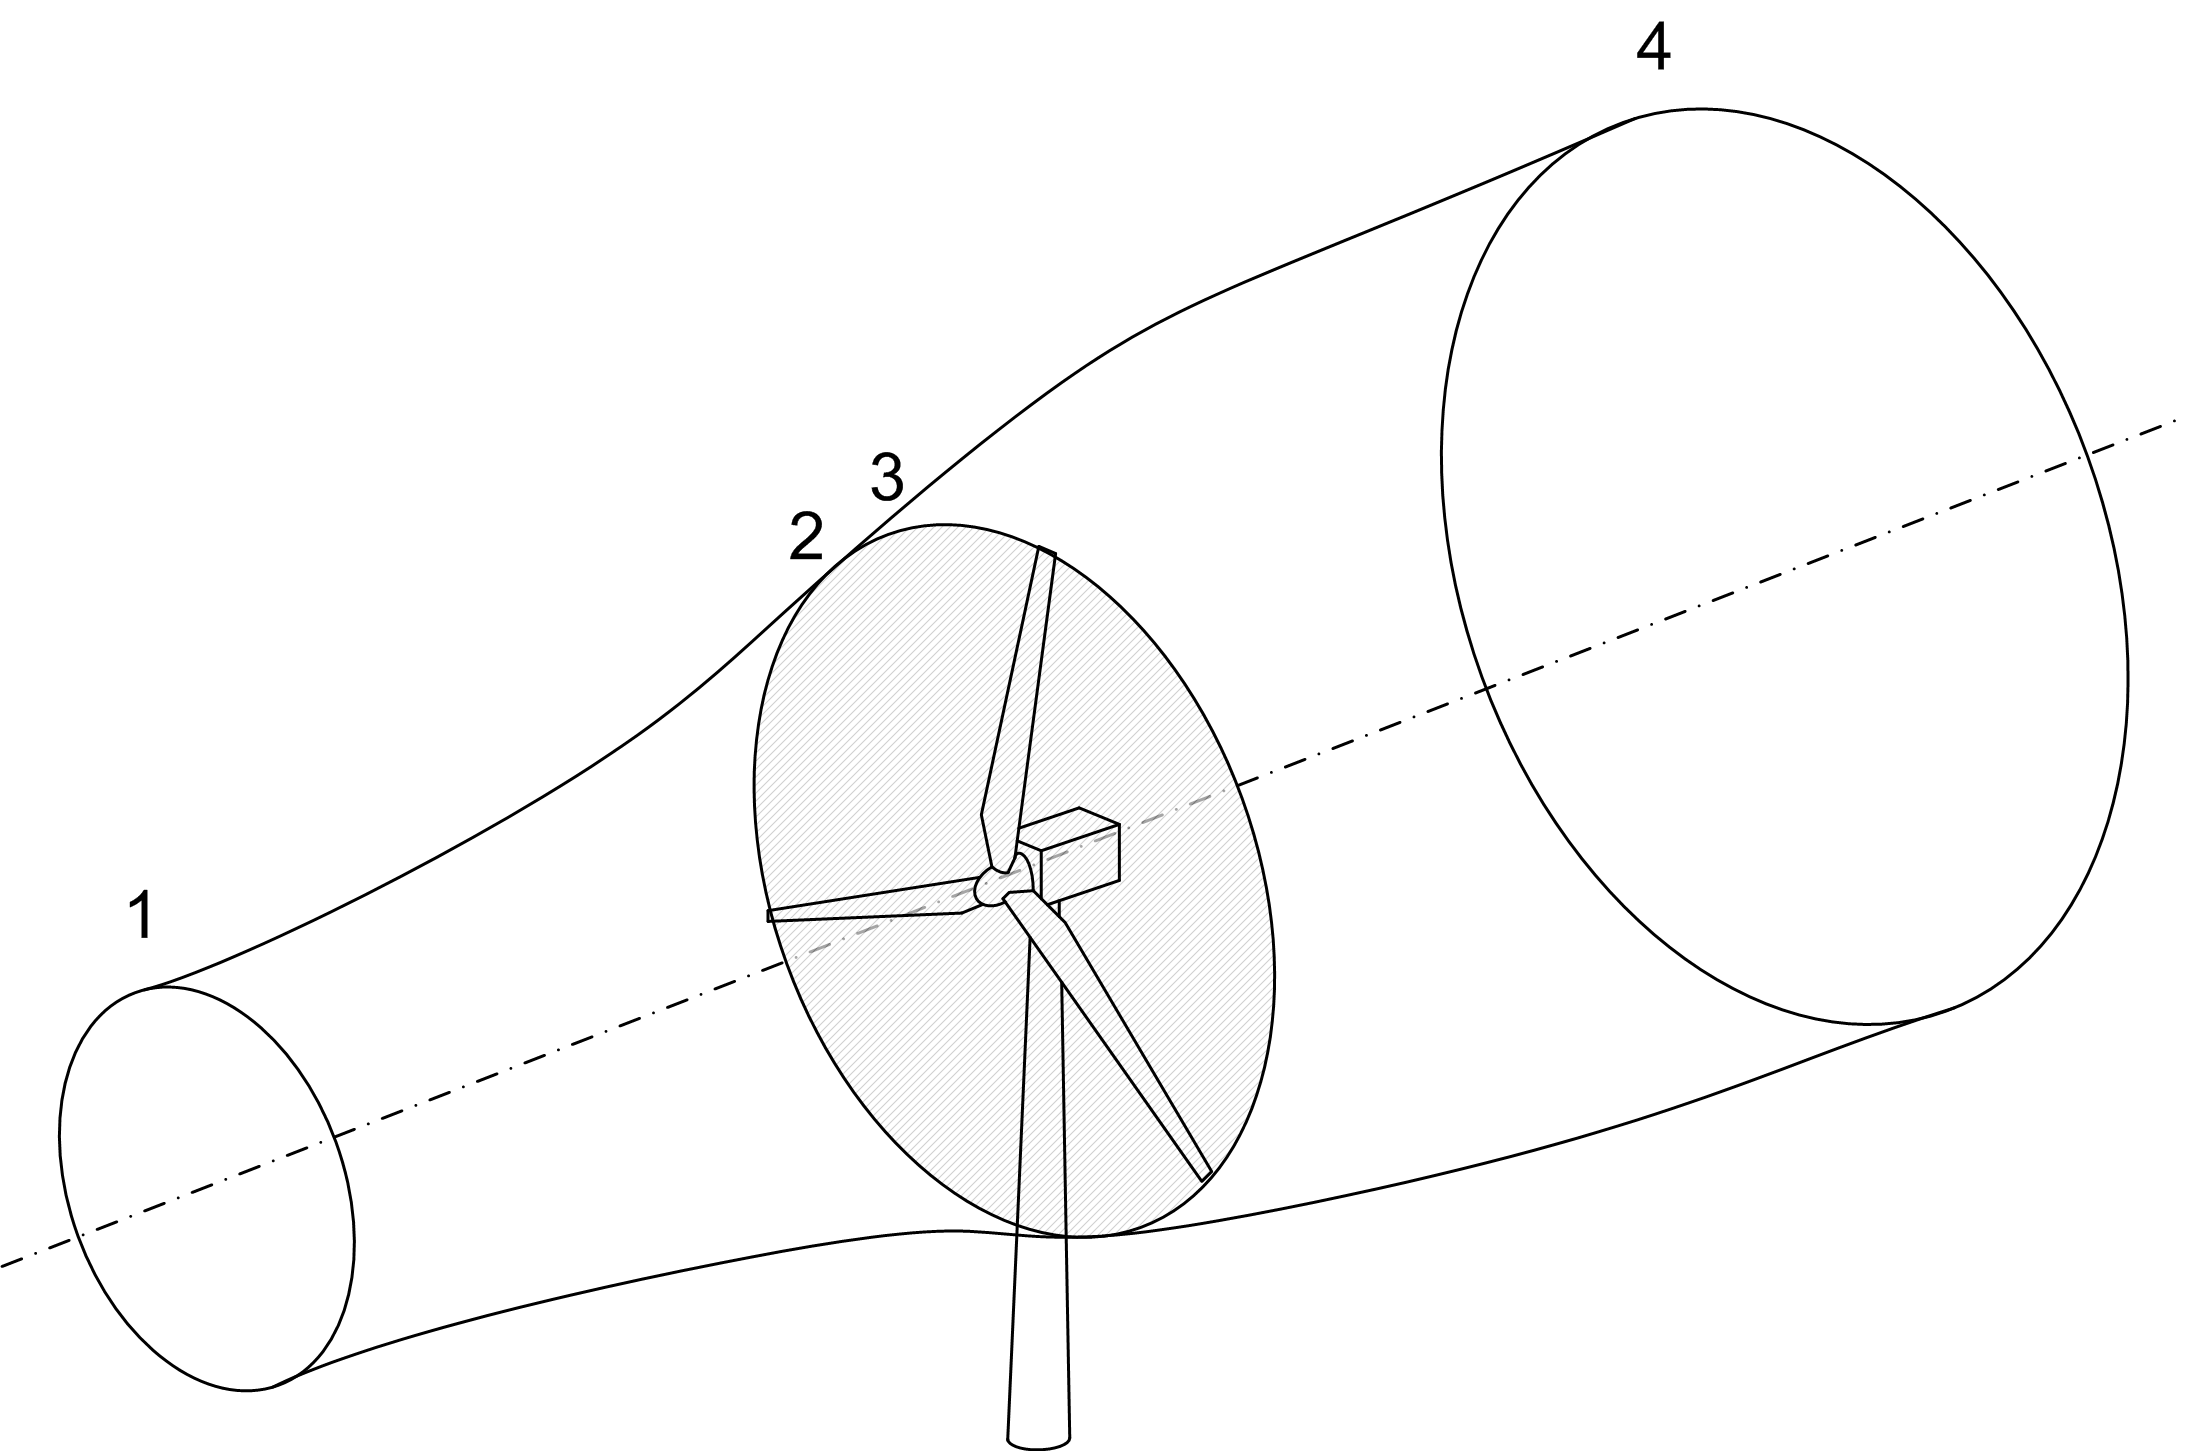
\includegraphics[width=0.6\linewidth]{../CIP_2/Figures/actuatordiskb.png}
\caption{Actuator disk model}
\label{fig:actuatordisk}
\end{figure}
Therefore we assume a closed system, which must obey momentum conservation. The rotor is moved by the incoming wind and angular momentum is induced. The wind is also influenced and is slowed down. The change in velocity is described by the induction factor $a$.
\begin{equation}
v_2 = v_1(1-a)
\end{equation}
In the following we first introduce the BEM algorithm and discuss some of the corrections which have to be consider when designing a wind turbine. It should be noted that these corrections are not used in the further design process because the application of the BEM is very complex and is done by specially designed programs.
\subsubsection{BEM algorithm}
The BEM algorithm is an iterative process and is limited by a convergence test. The following figure shows the main idea of the BEM algorithm.
\subsubsection{Prandtl factor}
The BEM theory by itself fails to represent all of the occurring effects which have to be considered. One major effect is the finite number of blades. The BEM theory calculates an uniform induction factor over each rotor ring, but in reality the local solidity decreases toward the tip and is not uniform over the ring. To deal with these errors the Prandtl correction is applied. The effects are shown in the following figure.

\begin{figure}[H]
\centering
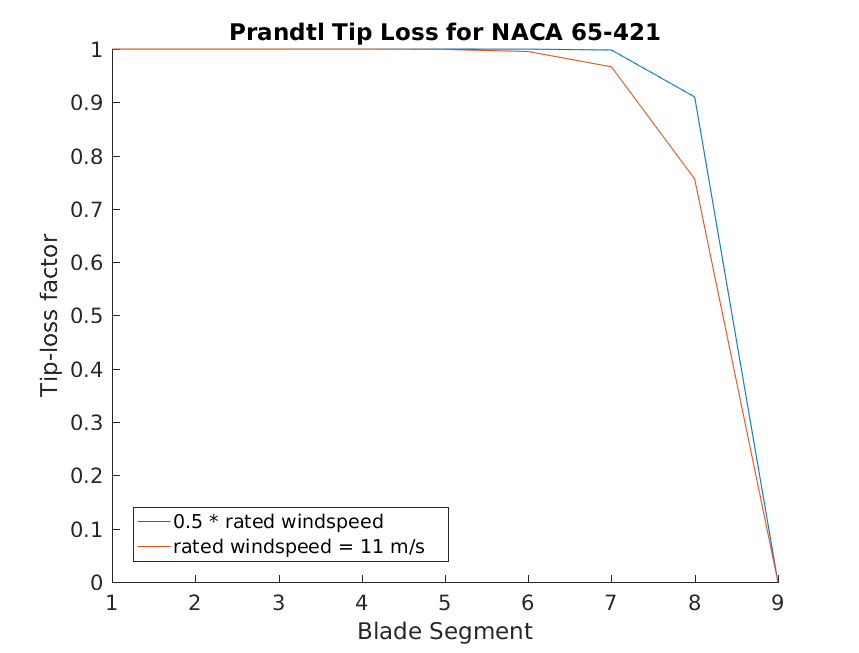
\includegraphics[width=0.8\linewidth]{../CIP_2/Figures/prandtl_tip_loss.png}
\caption{Prandtl Tip los}
\label{fig:tiplos}
\end{figure}

The figure shows that the tip-loss factor decreases with increasing r/R ratio. There are not big differences for alternating wind speeds. However it seems that higher wind speeds have a slightly bigger influence on the tip losses.

\subsection{3D corrections}
Measurements show that sometimes stall turbines have significant higher power in stall range than calculated. This is due to 3D effects which are not considered by 2D models. To deal with this problem, different corrections terms can be applied.
In the following two different models are shown. Figure~\ref{fig:hansen} shows the correction by Chaviaropoulus and Hansen and figure~\ref{fig:snel} the correction by Snel. 

\begin{figure}[H]
\centering
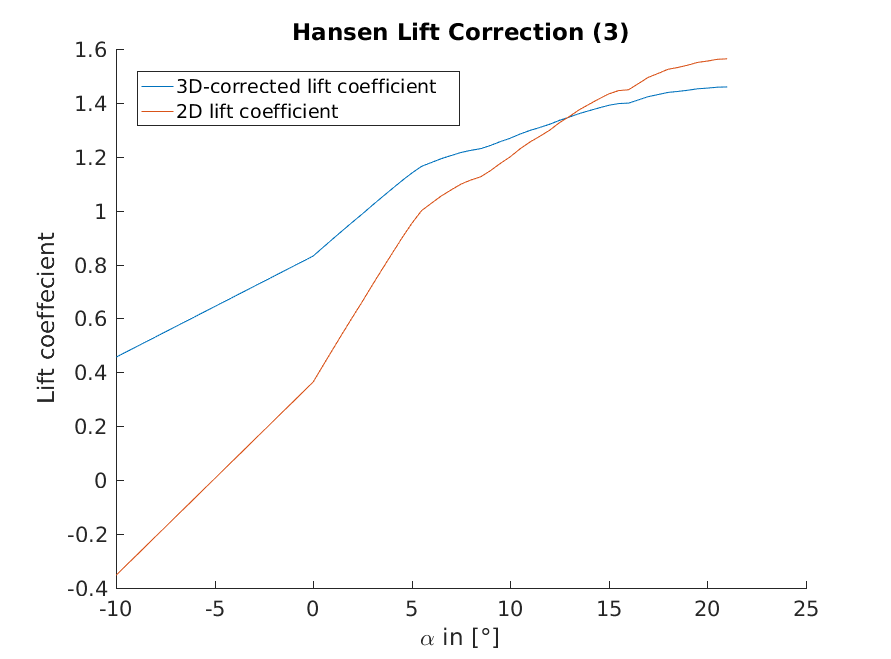
\includegraphics[width=0.8\linewidth]{../CIP_2/Figures/hansen_lift_correction_3.png}
\caption{Hansen 3D Correction}
\label{fig:hansen}
\end{figure}

\begin{figure}[H]
\centering
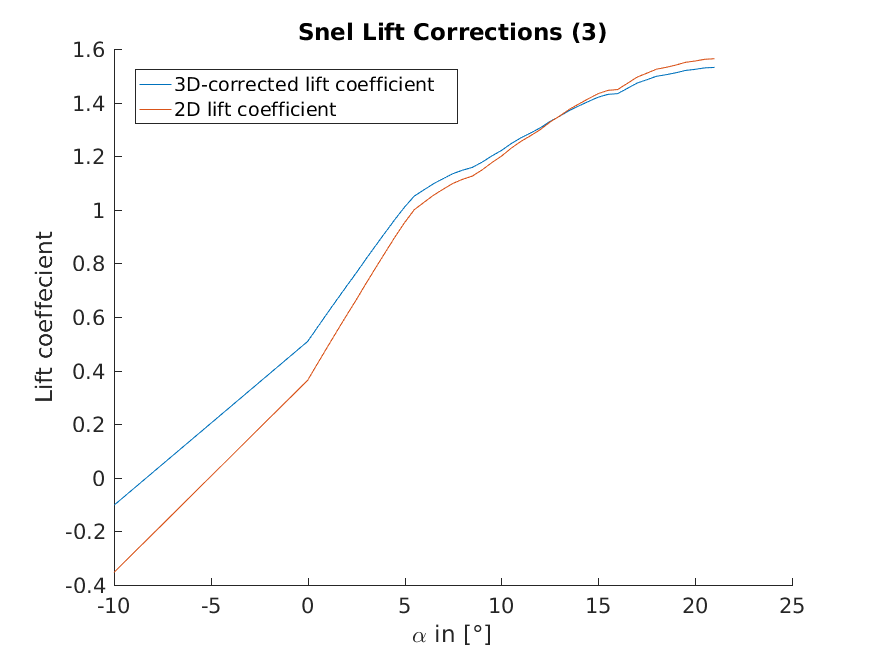
\includegraphics[width=0.8\linewidth]{../CIP_2/Figures/snel_correction_3.png}
\caption{Snel 3D correction}
\label{fig:snel}
\end{figure}

\subsection{Pitching moment}
We calculated the pitching moment at the different blade elements according to the following formula:
\begin{equation*}
M= C_m \cdot A \cdot c \cdot \rho \cdot v^2 \cdot 0.5
\end{equation*}
The total pitching moment can be obtained by adding up the moments of all blade elements. The results for the two different wind speeds ($v_{rated}$ and $0.5v_{rated}$}) are as follows:
\begin{align*}
M(5.5m/s) &= 15.881 Nm\\
M(11m/s) &= 278.705 Nm
\end{align*}

Figure~\ref{fig:pitchingcoeffs} depicts the pitching coefficients in dependance of the angle of attack.
\begin{figure}[H]
\centering
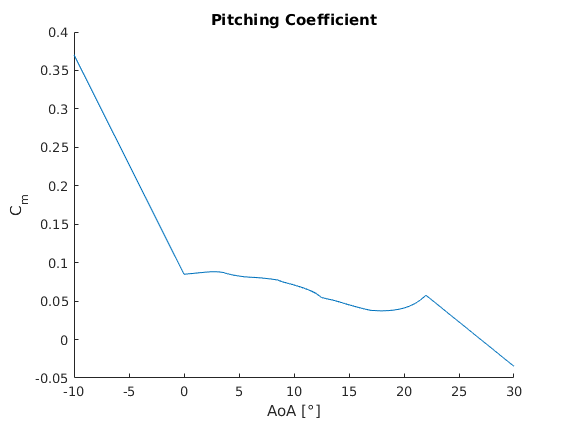
\includegraphics[width=0.8\linewidth]{../CIP_2/Figures/pitchingcoeff.png}
\caption{Pitching coefficient}
\label{fig:pitchingcoeffs}
\end{figure}


\newpage
\section{CIP 3: Performance Curves}
\subsection{Introduction}
In this section we analyzed the designed turbine under different pitch angles and tip-speed ratios. The design process of a wind turbine differs from turbine to turbine. In order to compare wind turbines non dimensional coefficients are used. These do not depend on factors like size or wind conditions. The most common coefficient is the power coefficient $c_p$. Further we used the torque coefficient $c_q$ and the thrust coefficient $c_t$.
These coefficient are defined as:
\begin{align*}
c_p = \frac{P}{0.5 *\rho A v^3}\hspace{0.5cm}c_t =  \frac{T}{0.5\rho A v^2}\hspace{0.5cm}c_q = \frac{Q}{0.5\rho A v^2*R}\\
\end{align*}
where:\\
$c_p$ = Power coefficient\\
$c_t$ = Thrust coefficient\\
$c_q$ = Torque coefficient\\
$p$   = Power\\
$\rho$ = Density\\
$A$    = Area\\
$v$	   = Wind speed\\
$R$		= Rotor radius

\subsection{WT\_Perf}
To compute the non dimensional parameters a program called WT\_Perf is used. 
WT\_Perf uses blade-element momentum (BEM) theory to predict the performance of wind turbines. \footnote{WT\_Perf\_Users\_guide.pdf}. It also takes different correction algorithms into account, e.g. Prandtl's tip-loss and hub-loss model.
WT\_Perf can be used from the operating system's command prompt. In order to use WT\_Perf  we configured the input file by updating the 'Turbine Data' section and implementing the calculated blade geometry. WT\_Perf also needs the aerodynamic data of the airfoils. We were able to use the provided data here. Last we defined the range of pitch angle and tip-speed ratio according to the tasks of CIP~3. \\
The following code-snippet gives an idea of the input file structure:
\newpage
\begin{lstlisting}
-----  Turbine Data  -----------------------------------------------------------
    3                NumBlade:                  Number of blades.
62.18                RotorRad:                  Rotor radius.
 1.25                HubRad:                    Hub radius. 
 -3.0                PreCone:                   Precone angle, positive downwind.
  5.0                Tilt:                      Shaft tilt.
  0.0                Yaw:                       Yaw error.
  100                HubHt:                     Hub height.
    8                NumSeg:                    Number of blade segments.

  RElm   Twist   Chord  AFfile  PrntElem
 3.808  26.530   6.988	 1	    FALSE
11.424	 9.594   5.407	 1      FALSE
19.040	 2.661   3.832	 1	    FALSE
26.656	-0.866	 2.906	 1	    FALSE
34.272	-1.967   2.171	 2	    FALSE
41.888	-3.354   1.806	 2	    FALSE
49.504	-4.335   1.544	 2	    FALSE
57.120	-5.066   1.348	 2	    FALSE
\end{lstlisting}

\subsection{Comparison}
As already mentioned we configured the input file according to CIP~3. The generated output file contains values for the power coefficient $c_p$, thrust $T$ and torque $Q$.
For task 3.2 we wrote a small python-program which examines the data and plots the results for the three different non dimensional coefficient mentioned in the introduction of CIP~3: $c_p, c_t$ and $c_q$. Since WT\_Perf only writes the power coefficient we had to calculate $c_t$ and $c_q$. Note that the coefficients are functions of $c_t(\lambda), c_q(\lambda)$.
The following figures display the results for $c_p, c_t$ and $c_q$ with a tip-speed ratio $\lambda$ from 1 to 20 and pitch angles of 0,5,10,15,20 and 30 degree. The curves are calculated at rated rotor speed (12.59 rpm).

\begin{figure}[H]
\centering
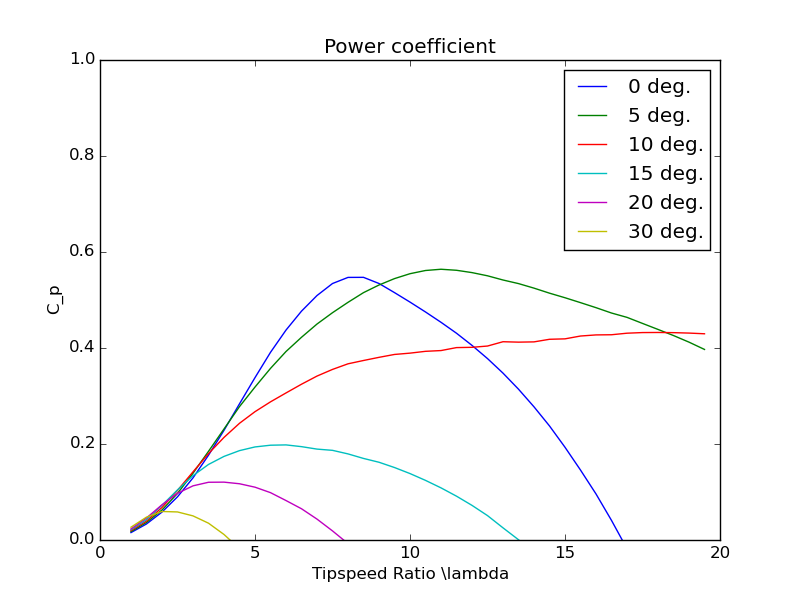
\includegraphics[width=1\linewidth]{../CIP_3/WT_Perf/Output/cp.png}
\caption{Power coefficient}
\label{fig:c-lambda}
\end{figure} 
The $c_p-\lambda$ curve shows different power coefficients at different tip-speeds and pitch-angles. Regarding the maximum for $c_p$ at each curve we identify that they appear at different tip-speed ratios. At pitch angle 5$^\circ$ the maximum $c_p$ is at 0.564 which is very close to the theoretical maximum of 0.592.

\begin{figure}[H]
\centering
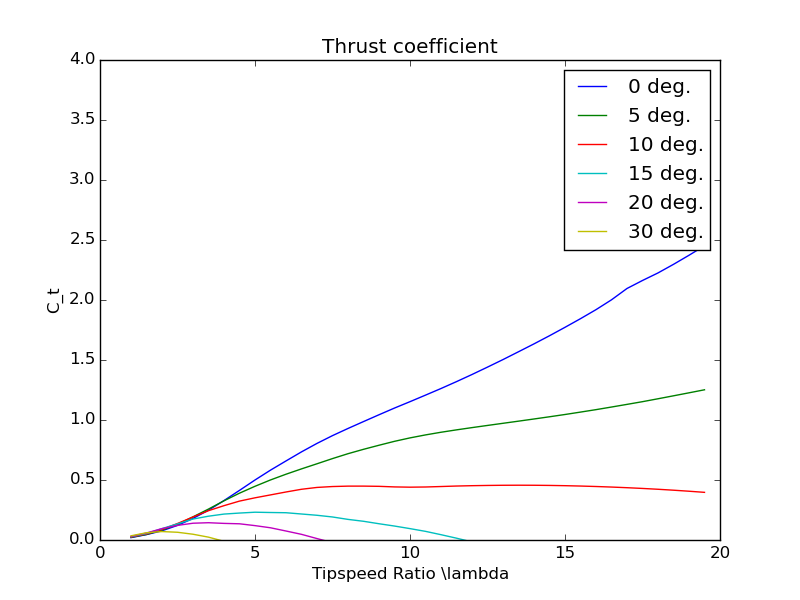
\includegraphics[width=1\linewidth]{../CIP_3/WT_Perf/Output/thrust.png}
\caption{Thrust coefficient}
\label{fig:thrust-coeff}
\end{figure} 
Figure \ref{fig:thrust-coeff} shows the behavior of the thrust coefficient. 
From 0$^\circ$ to 10$^\circ$ the thrust coefficient reaches high values. For higher pitch angles the resulting thrust coefficient is significantly lower and is equal to zero for higher tip speed ratios. The thrust is directly applied at the tower and can be decreased by increasing the pitch angle.

\begin{figure}[H]
\centering
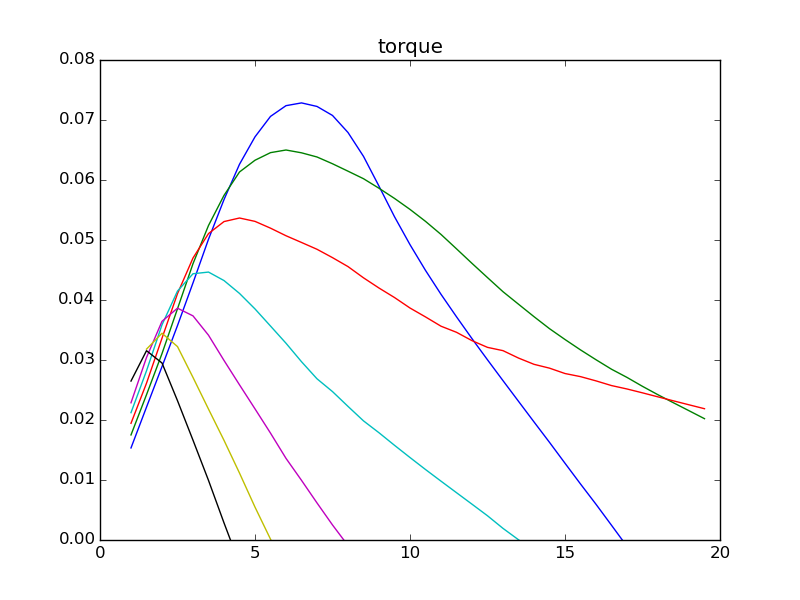
\includegraphics[width=1\linewidth]{../CIP_3/WT_Perf/Output/torque.png}
\caption{Torque coefficient}
\label{fig:torque-coeff}
\end{figure} 
Figure \ref{fig:torque-coeff} shows the torque coefficient for different pitch angles. Compared to the $c_p-\lambda$ the maximums are shifted to the left and decrease with increasing pitch angle.  

In the following the simulated results are compared to the corresponding curves from the literature\footnote{Gasch, R.: Wind Power Plants - Fundamentals, Design, Construction and Operation, 1st Edition, Solarpraxis AG, Berlin, 2002}. Figure~\ref{fig:power-coeff-lit} shows a power curve from literature. The maximum $c_p$ is close to 0.52 at zero degree pitch and design tip speed ratio. The results from figure~\ref{fig:c-lambda} is somewhat similar with the maximum at 0.554. Also the shape of pitch angles 0, 10, 20 and 30 degree of the designed turbine have a similar shape compared to the power curve from the literature. The designed turbine seems to overestimate the $c_p$ for higher tip speed ratios at pitch angle $5^{\circ}$ and $10^{\circ}$. According to the literature lower $c_p$ values should be assumed.


\begin{figure}[H]
\centering
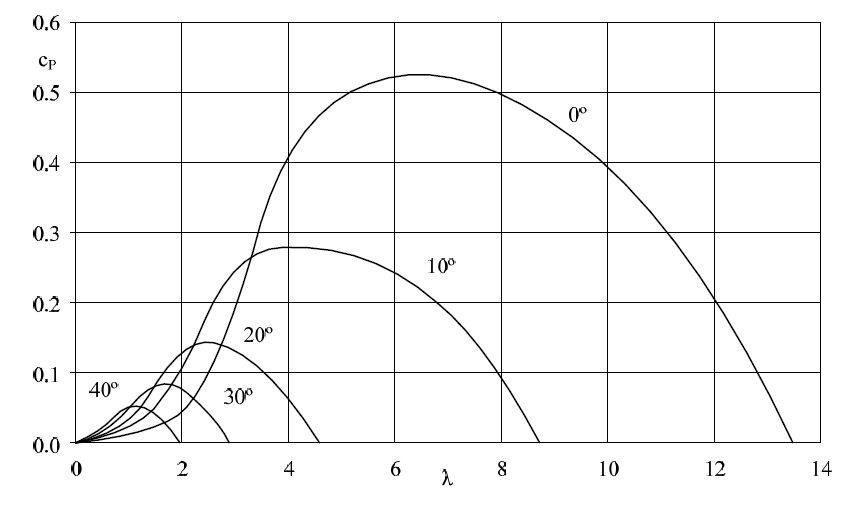
\includegraphics[width=1\linewidth]{../CIP_3/Report/power_coeff_literature.png}
\caption{Power coefficient from literature}
\label{fig:power-coeff-lit}
\end{figure} 

The same comparison has been done for the thrust coefficient. Figure~\ref{fig:thrust-coeff-lit} shows the expected outcome predicted by the literature. It can be seen that the thrust coefficient for the designed turbine looks very similar in it's shape compared to the thrust coefficient shown in figure~\ref{fig:thrust-coeff-lit}. For high pitch angles the curve reaches zero quickly. Lower pitch angles lead to an increasing thrust coefficient for higher tip speed ratios.

\begin{figure}[H]
\centering
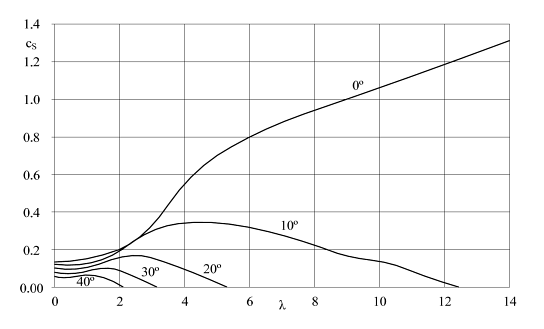
\includegraphics[width=1\linewidth]{../CIP_3/Report/thrust_coeff_literature.png}
\caption{Thrust coefficient from literature}
\label{fig:thrust-coeff-lit}
\end{figure} 

At last the predicted torque coefficient was evaluated in figure \ref{fig:torque-coeff-lit}. The designed turbine shows the same deviation that was already seen in the power curve. Pitch angles 5 and 10 degree seem to be a little bit off for higher tip speed ratios. 

\begin{figure}[H]
\centering
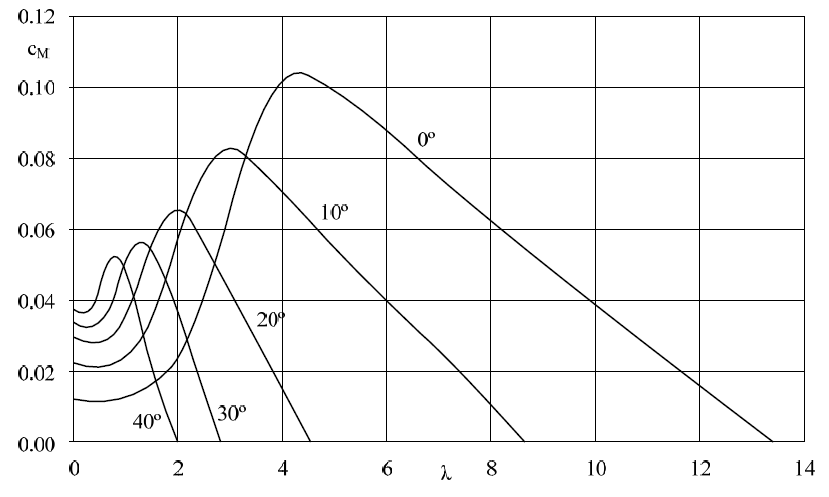
\includegraphics[width=1\linewidth]{../CIP_3/Report/torque_coeff_literature.png}
\caption{Torque coefficient from literature}
\label{fig:torque-coeff-lit}
\end{figure} 

\subsection{Rotor rated speed}
In task 3.4 we were asked to calculate the resulting rotor speed for a rated wind speed of 9 m/s. For the calculation we used our design tip speed ratio:
\begin{align}
\lambda = \frac{\Omega R}{v}\\
n = \frac{60 \lambda v}{2 \pi R} = 10.07 rpm
\end{align}
\subsection{Operation conditions}
Again we used WT\_Perf to calculate the resulting operation conditions below rated wind speed. The input parameters are: v = 9 m/s, design top speed ratio $\lambda$ = 8.2 and rotational speed $n$ = 10.07 rpm. The results are shown in the following table:\\

\begin{tabular}{|c |c| c| c| c| c|}
\hline
v & rotor speed & $c_p$ & $c_t$ & $c_q$ & $P$\\
m/s &rpm & - &- &-& kW\\
\hline
9 &10.07&0.544&0.825&0.033& 2054.846\\
\hline
\end{tabular}
\subsection{Coefficients}
According to Betz, the wind turbine should be able to extract 7618 kW.
However the rated power of the wind turbine is lower than the power which could be extracted. Therefore pitching is needed. The resulting $c_p$ can be calculated as follows:
\begin{equation}
c_p = \frac{3500000}{0.5 \cdot 1.225 \cdot \pi\cdot  62.18^2 \cdot  12^3} = 0.272
\end{equation}

\begin{figure}[H]
\centering
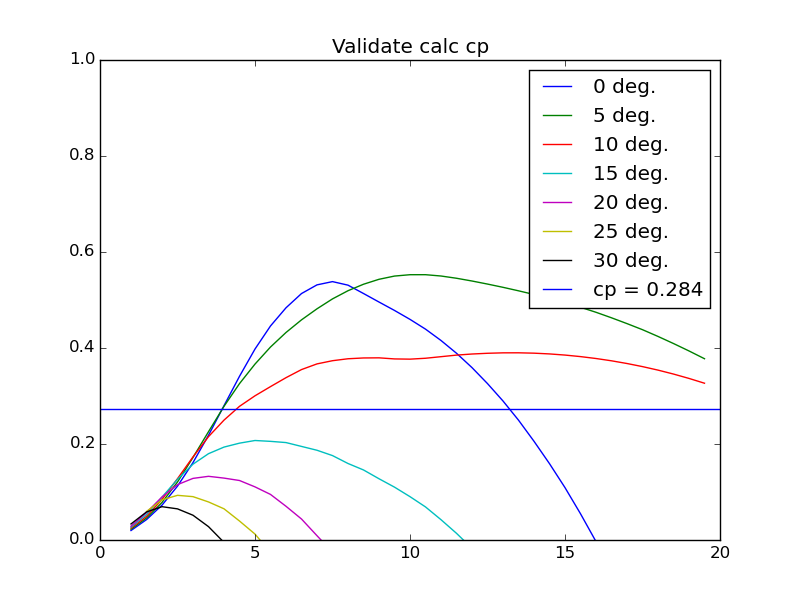
\includegraphics[width=1\linewidth]{../CIP_3/WT_Perf/Output/validated_cp.png}
\caption{Validation of $c_p$}
\label{fig:validate}
The resulting $c_p$ corresponds to a tip speed ratio of 5 with a pitch angle of 10$^\circ$
\end{figure} 
\subsection{Rotor speed}
\begin{align*}
n = \frac{60 \lambda v}{2 \pi R} = 9.21 rpm
\end{align*}
It can be seen, that for conditions below rated wind speed it is still possible to achieve a high power coefficient. The calculated power coefficient for 9 m/s is 0.544. If the wind speed is higher than the rated wind speed the power coefficient drops significantly. This is due to the limited capacity of the generator. Not all kinetic energy of the wind can be transformed into electrical energy and pitching is required to protect the generator. 
In both cases the rotations per minute are below rated rotor speed. Therefore the most efficient possibility to design a turbine is to make it variable. A constant tip speed ratio can be achieved, which leads to a high power coefficient.
\newpage
\section{CIP 4: Tower design}

In this part of the Design project a modal analysis for tower design will be carried out and evaluated with respect to economical factors. For this purpose the following parameters are relevant:

\begin{align*}
	\Omega_{rated} &= 14.5 rpm \text{ (rotor rated speed)} \\
	D &= 5m \text{ (tower diameter)} \\
	E &=211000000000 \frac{N}{m^2} \text{ (elastic modulus)} \\
	l &=100m \text{ (hub height)} \\
	m_{top} &=323000 kg\text{ (nacelle and rotor mass)} \\
	\rho &=7850 \frac{kg}{m^3}\text{ (material density)} \\
\end{align*}

\subsection{Eigenfrequency}
For tower design resonances of excitation frequencies from the rotating blades must be taken into account. The Eigenfrequency of the tower can thus be obtained by adding a $10 \%$ safety margin to the rotor rated speed which represents the maximum stationary rotor speed:
\begin{equation*}
	f_0 = \Omega_{rated} \cdot 1.1 = \frac{14.5}{60} Hz \cdot 1.1 = 0.2658 Hz
\end{equation*}

\subsection{Design range}
The design range of our turbine is a classical soft-stiff design which results in large wave excitation but allows variable speed turbine design since resonances with tower eigenfrequencies at frequencies lower than rated rotor speed are avoided. There are a few other common design approaches one of which is the soft-soft design where the eigenfrequency lies within the resonance range of the rotor. In this case certain rotor frequencies have to be excluded in order to avoid resonances.

\subsection{Wall thickness}
The wall thickness $t$ can be computed from the following equations:

\begin{align}
f_0 \cdot 2 \pi &= \sqrt{\frac{k}{m_{top} + 0.25 m_{tower}}} \\
k &= \frac{3 E \pi D^3 t}{l^3 8} \\
m_{tower} &= \rho \pi D t l
\end{align}

By substituting Equations (22) and (23) into (21) we obtain the following equality which can be fed into Matlab in order to solve for the only unknown $t$:\\

\begin{equation*}
0 = \sqrt{\frac{3 E \pi D^3 t}{l^3 8 \cdot (m_{top} + 0.25\rho \pi D t l)}} -f_0 \cdot 2 \pi \\
\end{equation*}

Extract from Matlab code used to solve for variable $t$:\\

\begin{lstlisting}
t=1;
func = @(t) sqrt(3*E*pi*D^3*t/(l^3*8*(mTop+0.25*rho*pi*D+t*l)))-f0*2*pi;
t = fsolve(func,t);
\end{lstlisting}

The resulting value for the wall thickness is $t=0.0318m$. The tower mass is then $m_{tower}=391730 kg = 391.73t$. The material cost for this tower would thus be of $195870$ \euro, assuming a price of $500$ \euro /t. Obviously a thicker tower wall leads to a higher price overall (linear increase). As depicted in Figure~\ref{fig:eigfreqWall} a thicker wall leads to a higher Eigenfrequency of the tower as well. However, in this case the relationship is not a linear one due to the exponent of $0.5$ in the formula. Hence, a thicker wall results in a higher Eigenfrequency but the increase is only significant for wall thicknesses up to $0.1m$. Above that the cost increase does not justify the gain in Eigenfrequency because wall thickness and costs are proportional but the Eigenfrequency is under-proportional.

\begin{figure}[H]
\centering
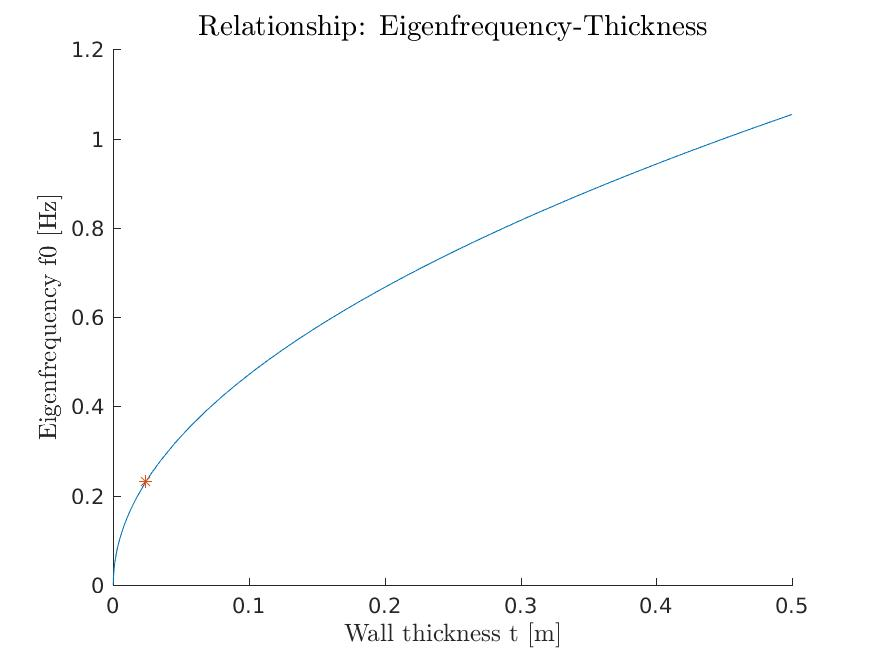
\includegraphics[width=\linewidth]{../CIP_4/figures/eigenfrequency.jpg}
\caption{Effect of wall thickness on Eigenfrequency}
\label{fig:eigfreqWall}
\end{figure} 

\subsection{Campbell diagram}
The Campbell diagram is depicted in Figure~\ref{fig:campbell}. The red line shows the computed Eigenfrequency of the tower and the circles mark resonance cases for certain rotor speed values due to periodic excitations. For example the dashed blue line ($1\Omega$) represents the 1P excitation (unbalance from the rotation), the second blue line ($3\Omega$) represents the periodic excitation caused by a tower shadow of one of the three blades.\\

The operational range of the rotor with respect to tower Eigenfrequencies must thus be kept within certain limits. By designing the tower wall thickness with adding a 10\% safety margin to the rotor rated speed we can are on the safe side and avoid 1P excitations (intersection point of the $\Omega$ line with the red line). It must further be excluded during operations that any of the other intersection points occur, e.g. $3\Omega$ line with red line. Some rotational speed ranges must thus be excluded in operation in order to avoid any resonances.This analysis however only considers tower resonances. A complete evaluation must take into account more resonances as well, e.g. 1st blade edgewise and 1st blade flapwise eigenfrequencies. \\

\begin{figure}[H]
\centering
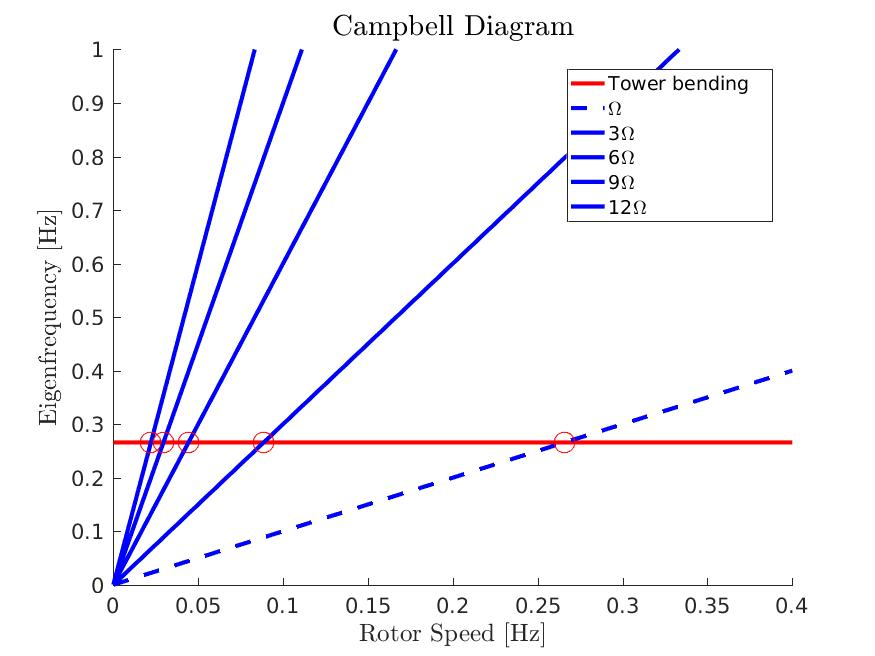
\includegraphics[width=1\linewidth]{../CIP_4/figures/campbell.jpg}
\caption{Campbell Diagram}
\label{fig:campbell}
\end{figure} 


\section{CIP 5: Wind fields and wake modeling}
\subsection{Wind speed distribution: Rayleigh}
Assuming a wind class type I-B gives per definition a reference wind speed of $V_{ref} = 50 m/s$ and a reference turbulence intensity of $I_{ref}=0.14$. The Rayleigh distribution as a special case of Weibull where the shape parameter has a value of $k=2$. The average wind speed can be derived from the reference wind speed as follows: $V_{ave}=V_{ref}/5 =10 m/s$. From this we can derive the scale parameter via $V_{ave} =  \lambda \cdot \sqrt{\frac{\pi}{2}}$ resulting in $\lambda = 7.97 m/s$. The corresponding wind speed distribution following a Weibull law with $\lambda = 7.97 m/s$ and $k=2$ is depicted in Figure~\ref{fig:rayleigh}. Frequencies were multiplied with 8760 in order to represent the absolute number of hours per year. Three crucial wind speeds are highlighted in the diagram: Cut-In speed ($3.5 m/s$), Rated speed ($11 m/s$) and Cut-Out speed ($25 m/s$). These three limits define the operational conditions of the turbine: Between Cut-In and Rated speed the turbine is operating in partial load, between rated speed and Cut-Out the turbine is operating under full load. Beyond these limits the turbine is not operating.

\begin{figure}[H]
\centering
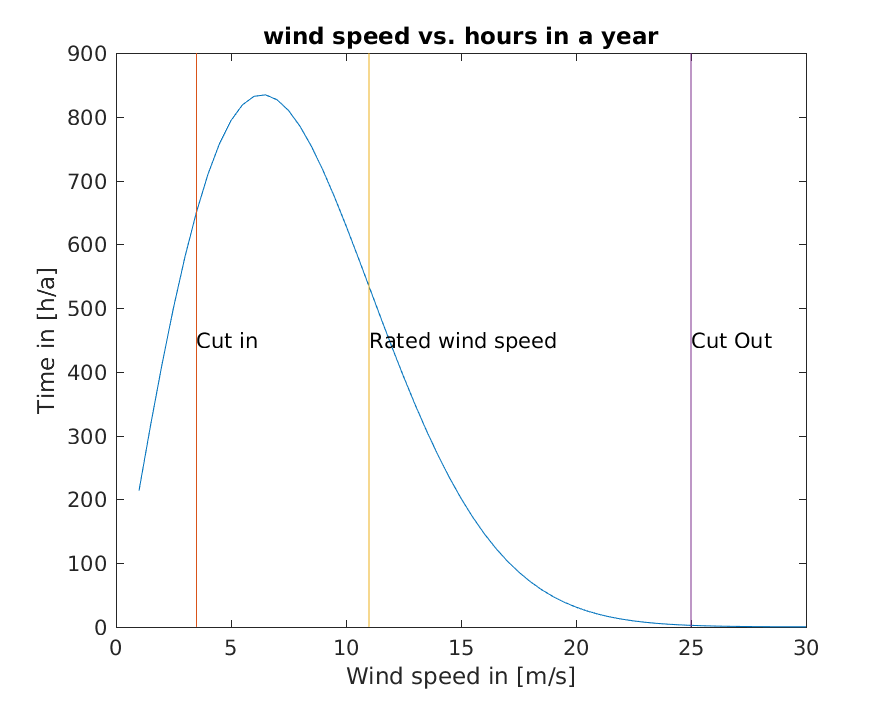
\includegraphics[width=1\linewidth]{../CIP_5/CIP_Tutorial_5_-_Windfield_and_wake_simulation/windspeed_vs_hours_year.png}
\caption{Wind speeds vs hours per year}
\label{fig:rayleigh}
\end{figure} 

\subsection{Power curve and AEP}
The power produced depending on the wind speed can be obtained from the following formula:
\begin{equation*}
P(v) = 0.5 \cdot \rho \cdot \nu \cdot \pi \cdot R^2 \cdot v^3
\end{equation*}
Wind density is fixed at $\rho= 1.225$, the total conversion efficiency is given as $\nu=0.4705$ and the rotor swept area is $\pi \cdot 54^2 m^2$. For wind speeds above rated wind speed the power output of the turbine will be constant.
The corresponding power curve is depicted in Figure~\ref{fig:powercurve}. 

\begin{figure}[H]
\centering
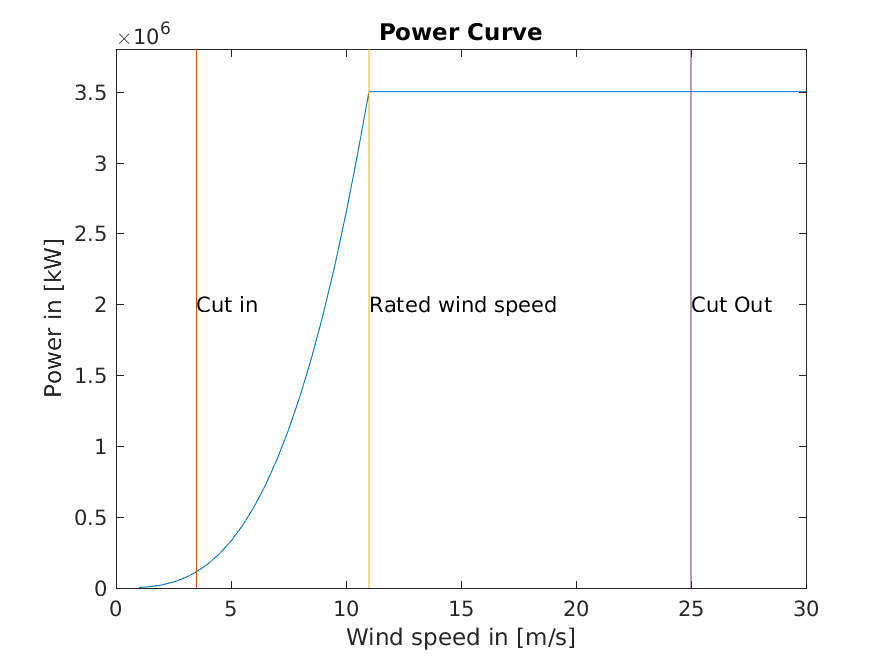
\includegraphics[width=1\linewidth]{../CIP_5/CIP_Tutorial_5_-_Windfield_and_wake_simulation/power_curve.png}
\caption{Power curve}
\label{fig:powercurve}
\end{figure} 

Combining the wind speed distribution from Figure~\ref{fig:rayleigh} and the power curve from Figure~\ref{fig:powercurve} enables computing the annual energy production. We multiply the number of hours for each wind speed with the power output at that specific speed and integrate this over all relevant wind speeds. The result corresponds to the area under the curve in Figure~\ref{fig:energyYield}. 

\begin{figure}[H]
\centering
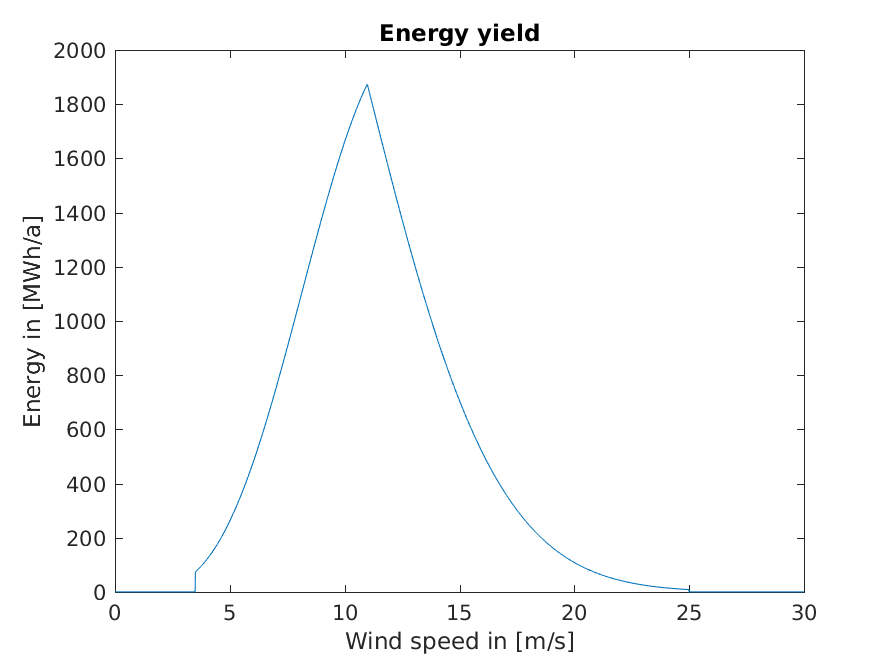
\includegraphics[width=1\linewidth]{../CIP_5/CIP_Tutorial_5_-_Windfield_and_wake_simulation/energy_yield.png}
\caption{Energy yield for different wind speeds}
\label{fig:energyYield}
\end{figure} 

Here, the total AEP is of about $11.099$ GWh. For a $100\%$ availability and a feed-in tariff of $0.08$~\euro/kWh the revenue is thus of approximately $887930$\euro. If we assume an availability of only $95\%$ the corresponding revenue lies around $843530$\euro which results in a loss of nearly $45000$\euro in one year.

\subsection{Turbulence intensity under free stream conditions}
Applying the normal turbulence model we calculated the turbulence intensity for different wind speeds. The wind class type is I-B which defines a reference intensity of $I_{ref}=0.14$. The result for the four given wind speeds is shown in Table~\ref{tab:freestream}.

\begin{table}[H]
\centering
\begin{tabular}{| c | c | c | c | c |}
\hline
\textbf{v} & $5m/s$ & $10m/s$ & $15m/s$ & $25m/s$ \\
\hline
\textbf{I} & $0.2618$ & $0.1834$ & $0.1573$ & $0.1364$	\\
\hline
\textbf{Operational condition} & partial & partial & full & full	\\
\hline
\end{tabular}
\caption{Turbulence intensity according to NTM at different wind speeds}
\label{tab:freestream}
\end{table}

From Figure~\ref{fig:energyYield} in the previous section we have seen that the biggest portion of the AEP of the turbine is contributed by wind speeds around rated wind speed. At higher wind speeds less energy is produced because these wind speeds simply are much less frequent due to the distribution, especially speeds of $20$m/s and higher are insignificant to the AEP. However, wind speeds around $5$m/s or $15$m/s do have an impact. Regarding the turbulence intensity shown above we can then conclude that there is no direct relation between turbulence and power output. 

\subsection{Wind fields with TurbSim}
Using TurbSim we generated wind fields for the given conditions, see Figure~\ref{fig:windfields}.

\begin{figure}[htb!]
\centering
\begin{subfigure}{0.4\textwidth}
  \centering
  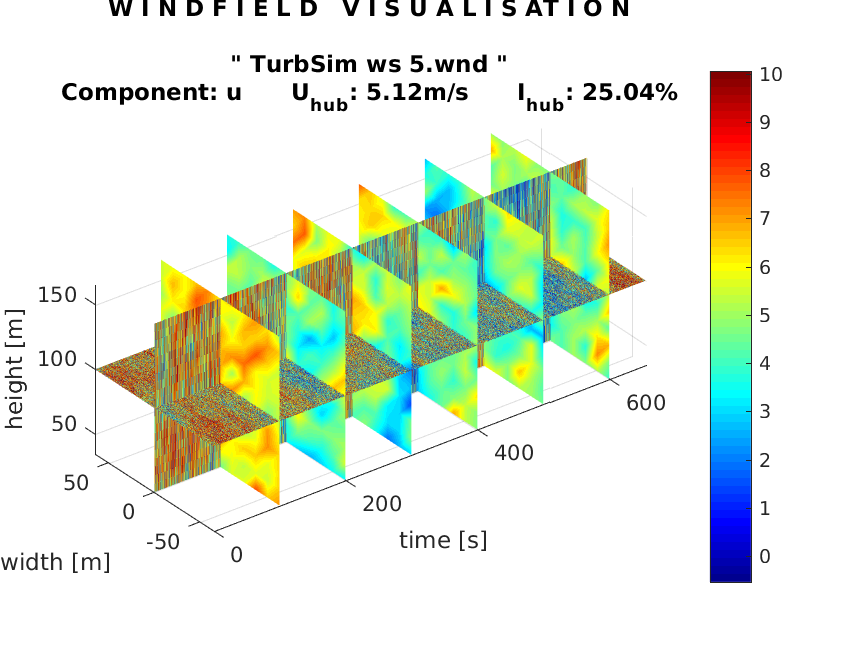
\includegraphics[width=1\linewidth]{../CIP_5/CIP_Tutorial_5_-_Windfield_and_wake_simulation/TurbSim/wind_5ms.png}
  \caption{At 5m/s}
\end{subfigure}
\begin{subfigure}{0.4\textwidth}
  \centering
  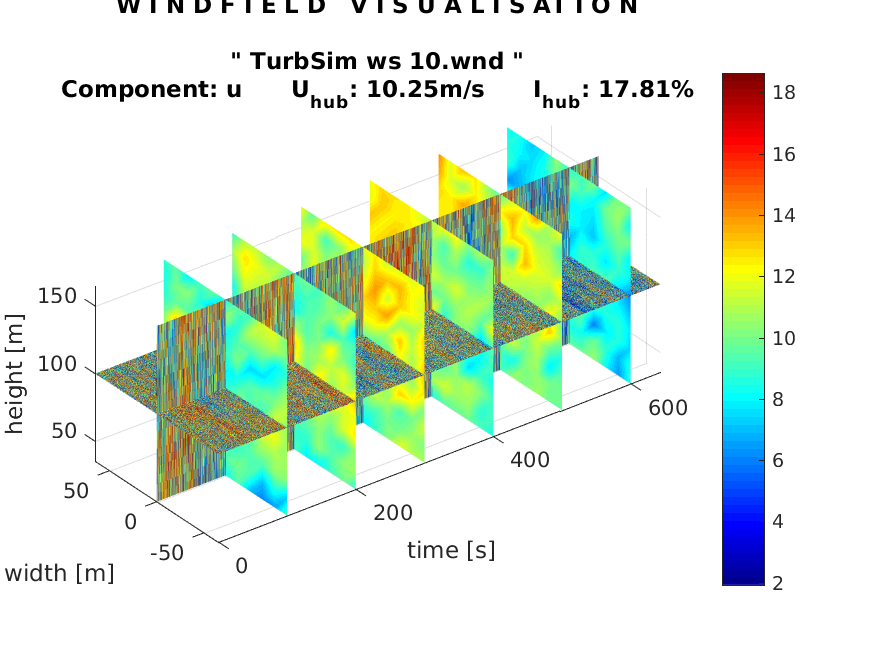
\includegraphics[width=1\linewidth]{../CIP_5/CIP_Tutorial_5_-_Windfield_and_wake_simulation/TurbSim/wind_10ms.png}
   \caption{At 10m/s}
\end{subfigure}
\begin{subfigure}{0.4\textwidth}
  \centering
  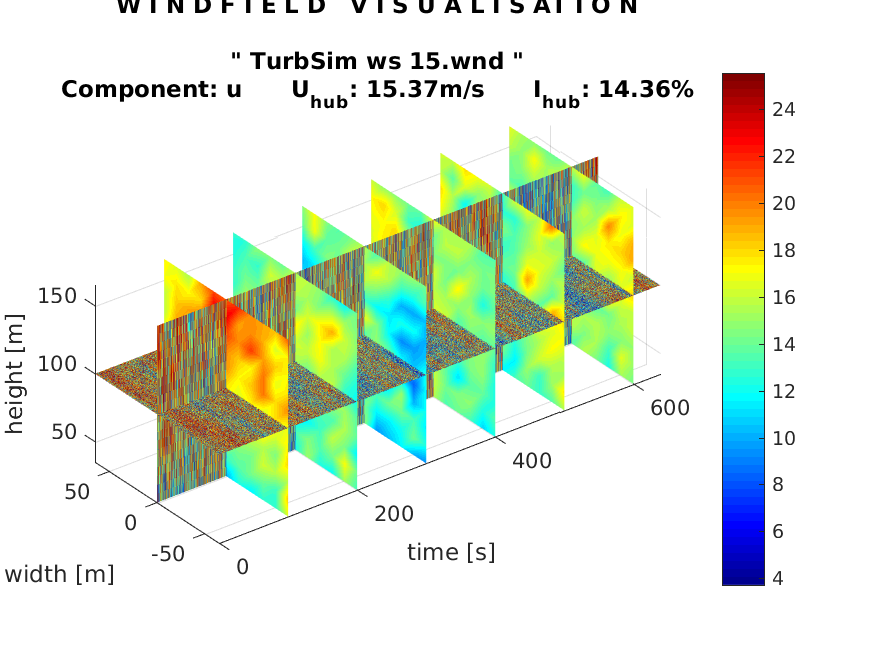
\includegraphics[width=1\linewidth]{../CIP_5/CIP_Tutorial_5_-_Windfield_and_wake_simulation/TurbSim/wind_15ms.png}
   \caption{At 15m/s}
\end{subfigure}
\begin{subfigure}{0.4\textwidth}
  \centering
  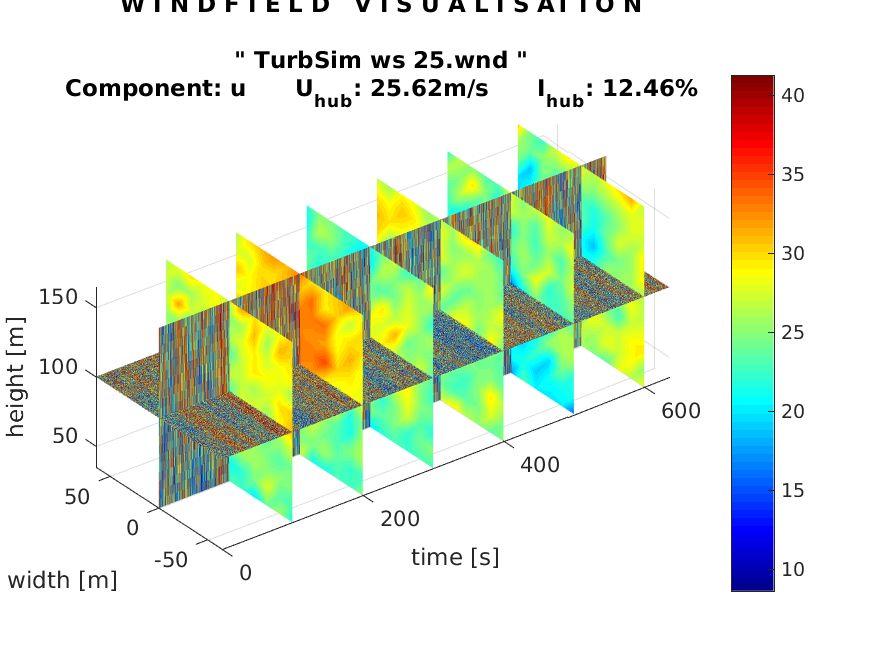
\includegraphics[width=1\linewidth]{../CIP_5/CIP_Tutorial_5_-_Windfield_and_wake_simulation/TurbSim/wind_25ms.png}
   \caption{At 25m/s}
\end{subfigure}
\caption{Wind fields by TurbSim}
\label{fig:windfields}
\end{figure}


\subsection{Wake modeling with Frandsen}
We now use Frandsen's model in order to analyze wakes. Two different setups will be evaluated: One with distances between the turbines of 4 times the rotor diameter, and one with 8 times the rotor diameter.
The result for the four given wind speeds is shown in Table~\ref{tab:waketable}. The results for the NTM model have been carried over in order to compare these to the wake results.
    
\begin{table}[H]
\centering
\begin{tabular}{| c | c | c | c | c |}
\hline
\textbf{v} & $5m/s$ & $10m/s$ & $15m/s$ & $25m/s$ \\
\hline
$\mathbf{4 \cdot d}$ & $0.2667$ & $0.1867$ & $0.1594$ & $ 0.1370$	\\
\hline
$\mathbf{8 \cdot d}$ & $0.2621$ & $0.1827$ & $0.1562$ & $0.1349$	\\
\hline
\textbf{NTM} & $0.2618$ & $0.1834$ & $0.1573$ & $0.1364$	\\
\hline
\end{tabular}
\caption{Turbulence intensity according to NTM at different wind speeds}
\label{tab:waketable}
\end{table}

Clearly the turbulence intensity is lower for the case of larger distances ($8 \cdot d$) for all wind speeds. However, the difference between the free stream turbulence and the case of larger distances is only marginal. For a wind speed of 5 m/s the turbulence intensity is lower in the free turbulence model, but for all other wind speeds the Frandsen model leads to lower turbulences then the free stream model. 

The complete dataset for all wind bins and all three cases is visualized in Figure~\ref{fig:turbintense}. It is not easy to recognize, but by looking closely we find that the order $8 \cdot d$, NTM, $4 \cdot d$ from lowest to highest turbulences holds for all wind bins above 10 m/s.

\begin{figure}[H]
\centering
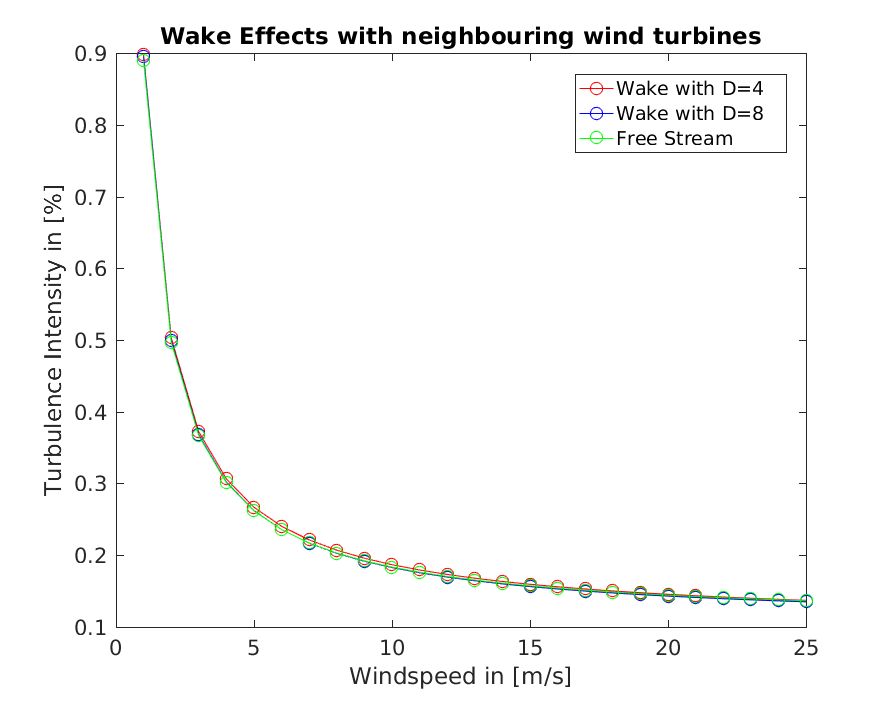
\includegraphics[width=0.5\linewidth]{../CIP_5/CIP_Tutorial_5_-_Windfield_and_wake_simulation/wake_effects_5.png}
\caption{Turbulence intensity in different setups}
\label{fig:turbintense}
\end{figure} 

We generated wind fields for wake conditions with both layouts as well since these will be used later. 
A comparison of the wind field under free stream conditions with the wind field under wake condition ($4\cdot d$) for $v=5m/s$ is shown in Figure~\ref{fig:windfieldsComp}. The two wind field do not diverge very much, but the computed turbulence intensity differs considerably ($0.2504$ vs $0.2544$).

\begin{figure}[htb!]
\begin{subfigure}{0.5\textwidth}
  \centering
  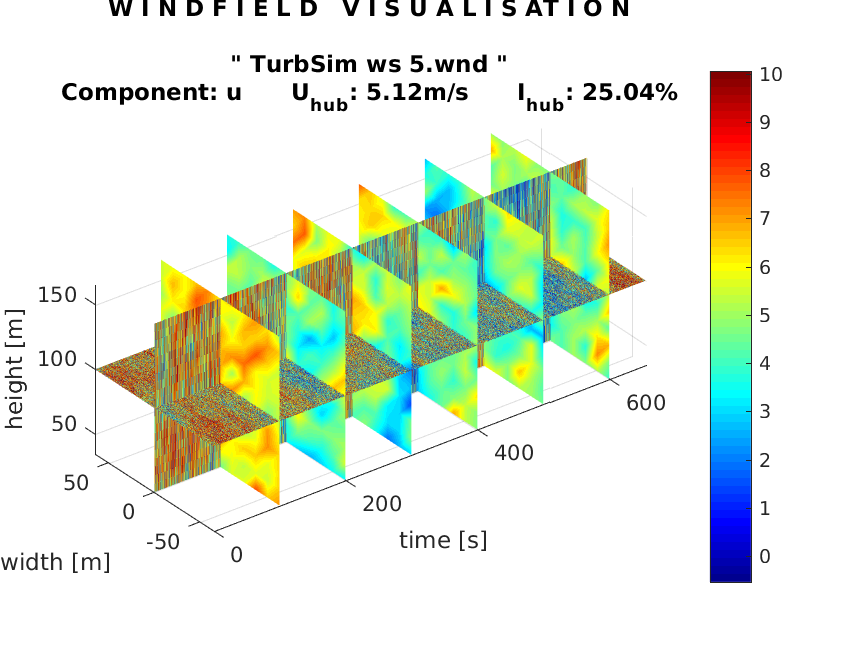
\includegraphics[width=1\linewidth]{../CIP_5/CIP_Tutorial_5_-_Windfield_and_wake_simulation/TurbSim/wind_5ms.png}
  \caption{Wind field for Free stream at 5m/s}
\end{subfigure}
\begin{subfigure}{0.5\textwidth}
  \centering
  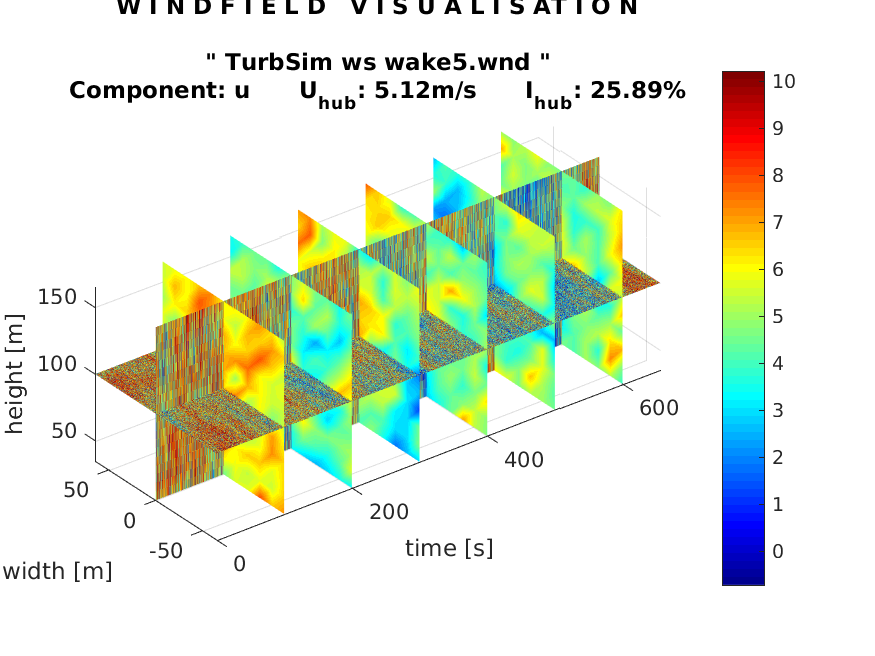
\includegraphics[width=1\linewidth]{../CIP_5/CIP_Tutorial_5_-_Windfield_and_wake_simulation/TurbSim/wind_wake_4_5ms.png}
   \caption{Wind field for Wakes with $4\cdot d$ at 5m/s}
\end{subfigure}
\caption{Free stream vs Wake conditions}
\label{fig:windfieldsComp}
\end{figure}

\subsection{Possible faults}
Failures can occur with respect to electrical components and the turbine control. These failures must be simulated in order to ensure structural integrity of the turbine. Possible faults are defect pitch or yaw actuators, which lead to the turbine being unable to reduce or increase forces and might cause a breakdown. Also it could be that sensors are defect and supply wrong data which would result in a fatal mis-behavior of the turbine. 
Likewise the drive train and gearbox might be affected by broken parts causing severe failure of the turbine if not handled correctly. The generator of a turbine can be subject to electromechanical problems, e.g. torque scaling fault, overheating, asymmetries etc.

\section{CIP 6a: Fatigue loads}
\subsection{FAST}
The wind fields from the previous chapter will now be used to run simulations with FAST for fatigue analysis.
We use the same wind speeds of 5,10,15 and 25m/s and free stream conditions. 

Figure~\ref{fig:bendingmoments5ms} shows the signals for the four variables (tower side-to-side, tower fore-aft, blade flapwise and blade edgewise) at a wind speed of $v=5m/s$. Units are kNm. The corresponding signals for higher windspeeds are analogue with a different scaling and different frequencies. 

We can see that the tower fore-aft bending moments are highest while side-to-side tower moments and blade edgewise moments are moderate. The oscillations are very regular in the case of the edgewise bending moments of the blade. For the other cases we see different maximums and minimums and some evolution in the course of the signal.

\begin{figure}[H]
  \centering
\begin{subfigure}{0.40\textwidth}
  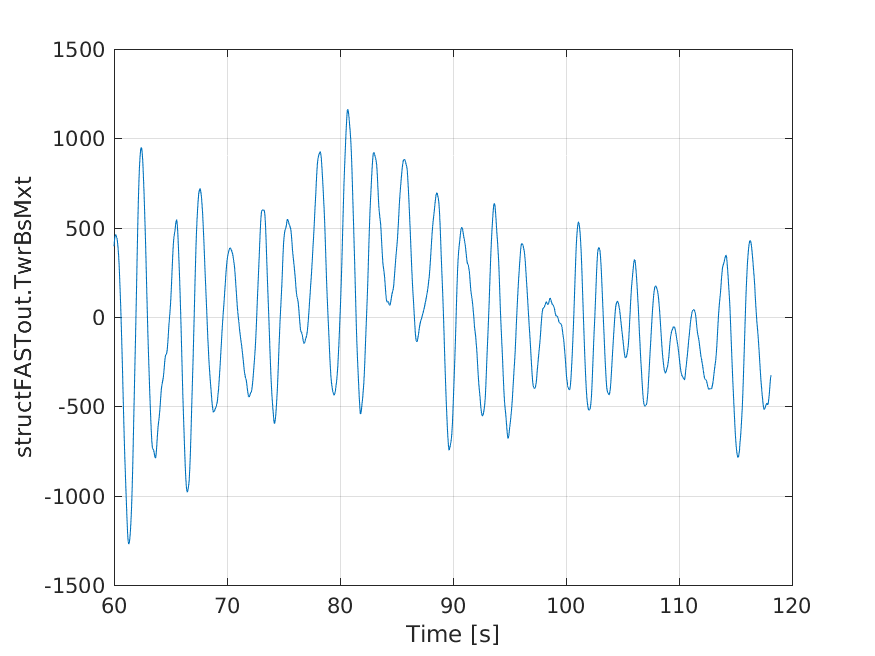
\includegraphics[width=1\linewidth]{../CIP_6/FAST/Plots_ws5/TwrBsMxt.png}
\caption{Tower side-to-side bending moments}
\end{subfigure}
\begin{subfigure}{0.40\textwidth}
  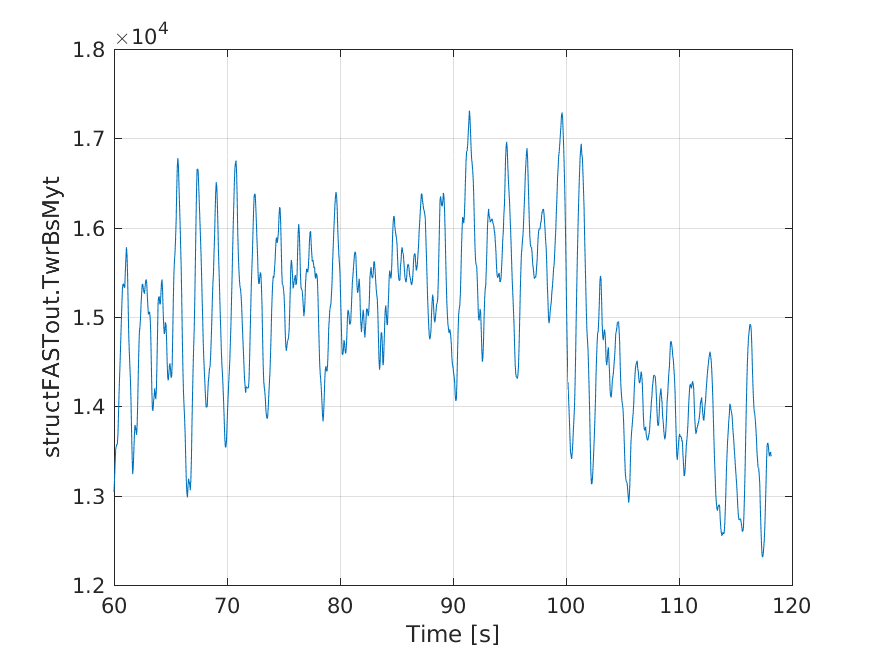
\includegraphics[width=1\linewidth]{../CIP_6/FAST/Plots_ws5/TwrBsMyt.png}
\caption{Tower fore-aft bending moments}
\end{subfigure}
\begin{subfigure}{0.40\textwidth}
  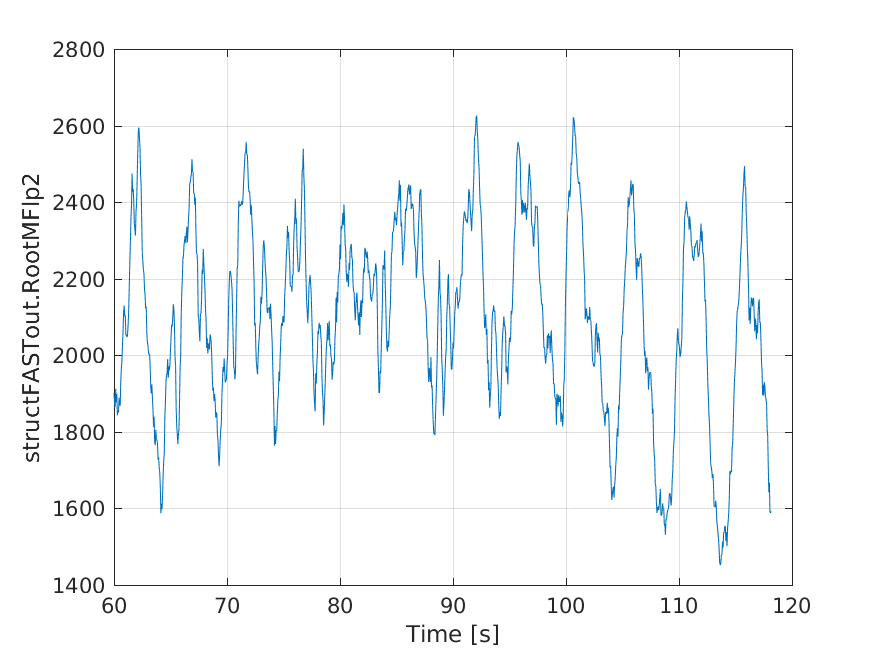
\includegraphics[width=1\linewidth]{../CIP_6/FAST/Plots_ws5/RootMFlp2.png}
\caption{Blade flapwise bending moments}
\end{subfigure}
\begin{subfigure}{0.40\textwidth}
  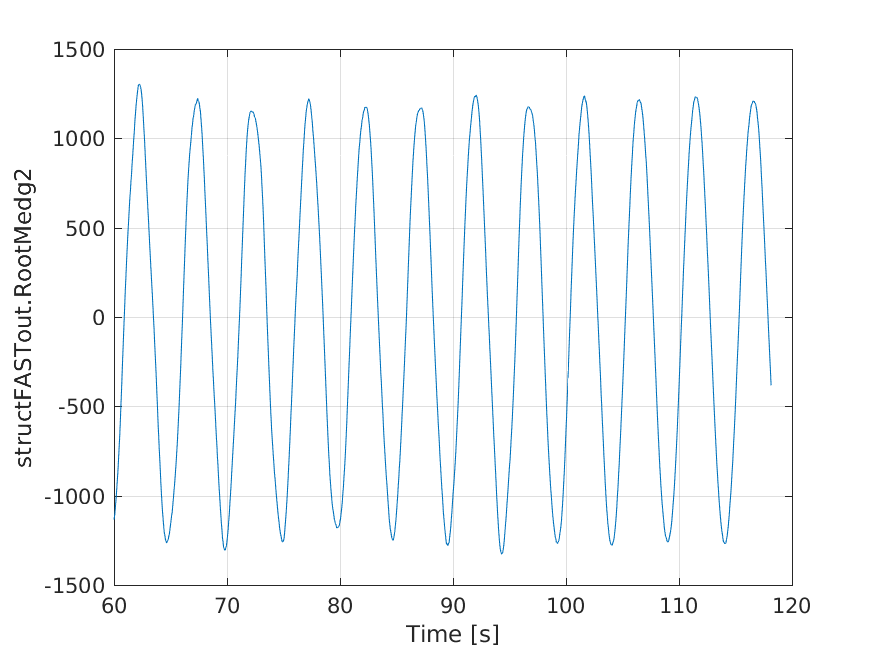
\includegraphics[width=1\linewidth]{../CIP_6/FAST/Plots_ws5/RootMedg2.png}
\caption{Blade edgewise bending moments}
\end{subfigure}
\caption{Time series of bending moments for different variables at $v=5m/s$}
\label{fig:bendingmoments5ms}
\end{figure}

\subsection{Damage equivalent loads under free stream condition}
The DELs under free stream conditions for tower and root can be found in Table~\ref{tab:DELfree}. Damage equivalent loads are used to represent the cyclic loads of a time series in one numeric value. We find confirmation for the result from the previous section: Highest loads occur in case of the tower fore-aft and edgewise blade bending moments. The loads increase with the wind speed over-proportionally for all variables. 

\begin{table}[H]
\centering
\begin{tabular}{| c | c | c | c | c |}
\hline
\textbf{v} & $5m/s$ & $10m/s$ & $15m/s$ & $25m/s$ \\
\hline
\textbf{Tower side-to-side} & $811.645$ & $1466.761$ & $2112.274$ & $4974.035$ \\
\hline
\textbf{Tower fore-aft} & $2382.669$ & $2990.821$ & $3862.967$ & $6328.944$	\\
\hline
\textbf{Blade edgewise} & $1924.045$ & $2387.446$ & $2432.449$ & $2552.909$	\\
\hline
\textbf{Blade flapwise} & $738.816$ & $1426.071$ & $1765.008$ & $2353.317$	\\
\hline
\end{tabular}
\caption{DELs under free stream conditions}
\label{tab:DELfree}
\end{table}


\subsection{Damage equivalent loads under wake condition}
The DELs under wake condition for tower and root can be found in Table~\ref{tab:DELwake}.

\begin{table}[H]
\begin{tabular}{| c | c | c | c | c |c | c | c | c |}
\hline
\multicolumn{1}{|c|}{\textbf{neighboring distance}} & \multicolumn{4}{c|}{$4\cdot d$} & \multicolumn{4}{c|}{$8\cdot d$} \\ 
\hline
\textbf{v} & $5m/s$ & $10m/s$ & $15m/s$ & $25m/s$ & $5m/s$ & $10m/s$ & $15m/s$ & $25m/s$ \\
\hline
\textbf{Tower side-to-side} & $775.607$ & $1404.149$ & $2087.209$ & $5419.259$ & $810.116$ & $1445.473$ & $2132.343$ & $5356.443$ \\
\hline
\textbf{Tower fore-aft} & $3050.375$ & $3695.06$ & $3620.304$ & $6162.187$ & $2651.542$ & $2677.856$ & $3516.175$ & $5957.573$	\\
\hline
\textbf{Blade edgewise} & $1940.040$ & $2419.468$ & $2416.637$ & $2555.216$ & $1923.647$ & $2397.627$ & $2436.092$ & $2560.151$	\\
\hline
\textbf{Blade flapwise} & $814.974$ & $1445.028$ & $1701.446$ & $2308.930$ & $791.422$ & $1351.939$ & $1721.214$ & $2299.36$	\\
\hline
\end{tabular}
\caption{DELs under wake condition}
\label{tab:DELwake}
\end{table}

Comparing the DELs in the three different settings (free stream and wake with $4\cdot d$ and $8\cdot d$) in Figure~\ref{fig:compDels} we can see that for the edgewise blade DELs there is no notable difference between the three settings. For the flapwise blade moments however the DELs are lowest for the setting with wakes and a $8\cdot d$ distance and highest for a $4\cdot d$ distance while the free stream setting lies in the middle.
Regarding the tower DELs the differences are more clear, especially in the case of fore-aft bending. Here again the $8\cdot d$ distance setting has lowest DELs at most wind speeds (except 5m/s) while the free stream setting has lower DELs then the $4\cdot d$ setting for moderate wind speeds.
The fact that the $8\cdot d$ distance case results in lower DELs then the $4\cdot d$ distance case is as expected as we saw in the previous chapter that the turbulence intensity is lower for the setting with larger distances between neighboring turbines. However, we would have thought that the free stream setting results in even lower DELs since the turbulence intensity was shown to be lower with the NTM model then in the Frandsen model. 

\begin{figure}[H]
  \centering
\begin{subfigure}{0.40\textwidth}
  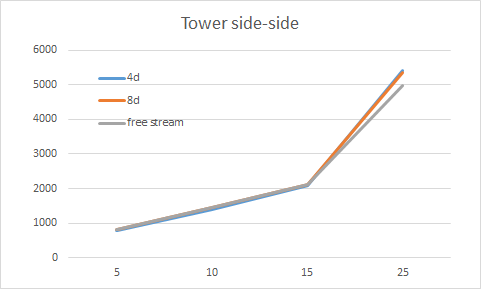
\includegraphics[width=1\linewidth]{figures/delsTwrSide.png}
\end{subfigure}
\begin{subfigure}{0.40\textwidth}
  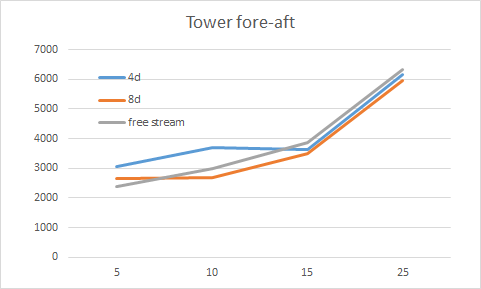
\includegraphics[width=1\linewidth]{figures/delsTwrFore.png}
\end{subfigure}
\begin{subfigure}{0.40\textwidth}
  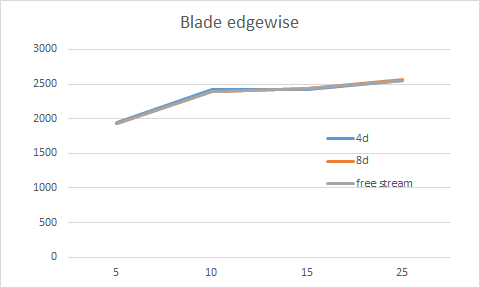
\includegraphics[width=1\linewidth]{figures/delsBldEdge.png}
\end{subfigure}
\begin{subfigure}{0.40\textwidth}
  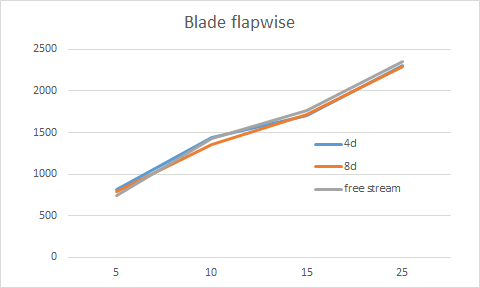
\includegraphics[width=1\linewidth]{figures/delsBldFlap.png}
\end{subfigure}
\caption{Comparison of the DELs}
\label{fig:compDels}
\end{figure}


\subsection{Statistical max/min sensor values}
The statistical max and min values of the sensors analyzed above for all settings can be seen in Table~\ref{tab:statmaxmin}.

\begin{table}[H]
\centering
\begin{tabular}{ | c | c | c | c | c | c | c | c | c | }
	 \hline
	 & \multicolumn{2}{c|}{Tower side-side} &  \multicolumn{2}{c|}{Tower fore-aft} & \multicolumn{2}{c|}{Blade flapwise} & \multicolumn{2}{c|}{Blade edgewise } \\
	 \hline
	 & Min & Max & Min & Max & Min & Max & Min & Max \\
	 \hline
	 NTM 5m/s & -1272 & 1163 & 12310 & 17310 & 1452 & 2626 & -1328 & 1304 \\
	 \hline
	 NTM 10m/s & -629.6 & 1635 & 9931 & 21010 & 778.8 & 3110 & -1678 & 1285 \\
	 \hline
	 NTM 15m/s & -2701 & 3865 & 4047 & 20430 & -306.5 & 3192 & -1798 & 1580 \\ 
	 \hline
	 NTM 25m/s & -8513 & 8904 & 732.7 & 23270 & -1855 & 2903 & -2001 & 1684 \\ 
	 \hline
	 4d, 5m/s & -1271 & 1504 & 4610 & 19290 & 1016 & 2861 & -1332 & 1314 \\ 
	 \hline
	 4d, 10m/s & -2666 & 2637 & 8794 & 40330 & 766.2 & 5109 & -1807 & 1775 \\ 
	 \hline
	 4d, 15m/s & -2481 & 3642 & 3418 & 19770 & -291.7 & 3247 & -1802 & 1609 \\ 
	 \hline
	 4d, 25m/s & -8523 & 9251 & 260.2 & 22730 & -1844 & 2894 & -1992 & 1710 \\ 
	 \hline
	 8d, 5m/s & -1183 & 1529 & 5393 & 19760 & 1024 & 2908 & -1330 & 1306 \\ 
	 \hline
	 8d, 10m/s & -2912 & 2818 & 8901 & 38050 & 774.3 & 4984 & -1866 & 1838 \\ 
	 \hline
	 8d, 15m/s & -2397 & 3576 & 3439 & 19730 & -272.9 & 3206 & -1804 & 1602 \\ 
	 \hline
	 8d, 25m/s & -8490 & 8621 & 1003 & 23480 & -1889 & 2921 & -2021 & 1684 \\ 
	 \hline
\end{tabular}
\caption{Max and mins of sensor values}
\label{tab:statmaxmin}
\end{table}



\subsection{Power spectral density}
For the blade flapwise bending moment and for the tower fore-aft bending moment under wake conditions (with $8\cdot d$ distance) the power spectral density plots can be found in Figure~\ref{fig:psdplots}. Two different wind speeds of 5 m/s and 25 m/s were chosen.
The overall pattern of the spectral density is similar in all cases. Frequencies below 1 Hz are most powerful but occur less then higher frequencies. Higher wind speeds leads to higher frequencies and flattens the spectral profile a little.

This tower was designed with an Eigenfrequency of $0.2658 Hz$. There is no obvious effect on the power spectral density of the Eigenfrequency. However, the power spectral density in all cases has these spikes which should be in same way linked to the Eigenfrequency of the system components, i.e. multiples of the blades flapwise and towers eigenfrequencies.

\begin{figure}[H]
  \centering
\begin{subfigure}{0.40\textwidth}
  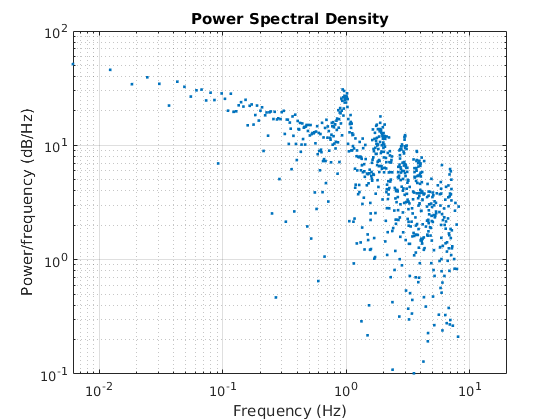
\includegraphics[width=1\linewidth]{../CIP_6/FAST/PSD_plots/PSD_ws5_wake8_BladeFlap.png}
    \caption{Blade flapwise at 5 m/s}
\end{subfigure}
\begin{subfigure}{0.40\textwidth}
  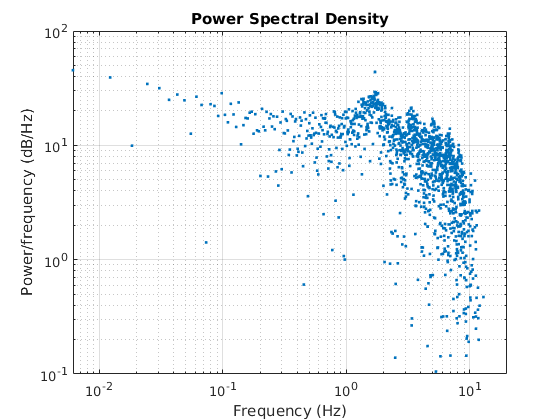
\includegraphics[width=1\linewidth]{../CIP_6/FAST/PSD_plots/PSD_ws25_wake8_BladeFlap.png}
      \caption{Blade flapwise at 25 m/s}
\end{subfigure}
\begin{subfigure}{0.40\textwidth}
  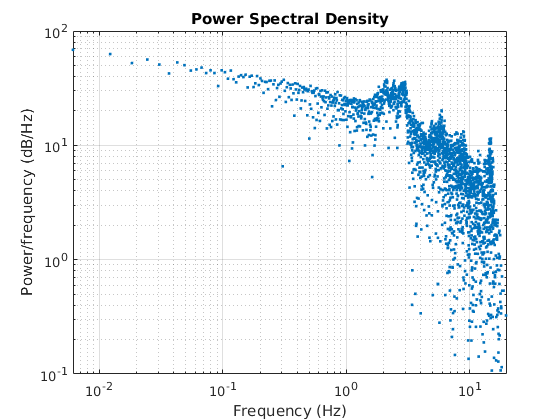
\includegraphics[width=1\linewidth]{../CIP_6/FAST/PSD_plots/PSD_ws5_wake8_TowerFore.png}
      \caption{Tower fore-aft at 5 m/s}
\end{subfigure}
\begin{subfigure}{0.40\textwidth}
  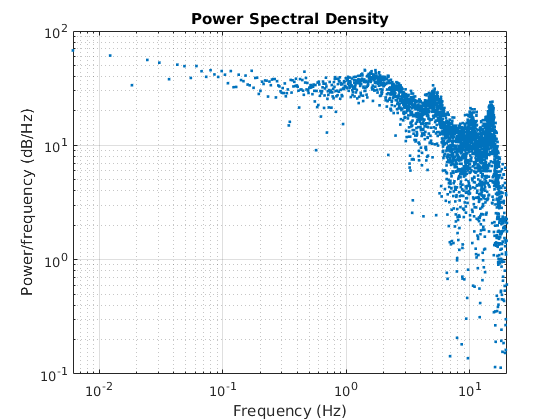
\includegraphics[width=1\linewidth]{../CIP_6/FAST/PSD_plots/PSD_ws25_wake8_TowerFore.png}
        \caption{Tower fore-aft at 25 m/s}
\end{subfigure}
\caption{Power spectral density plots}
\label{fig:psdplots}
\end{figure}


\section{CIP 6b: Extreme loads}
\subsection{Extreme conditions}
\begin{itemize}
\item Load case 1.3: \\
	Power production under the ETM (extreme turbulence model). This load case is important because extreme turbulences can damage the turbine's components much more than normal turbulence which reduces lifetime. These conditions must thus be simulated 
\item Load case 1.5: \\
	Power production under the EWS (extreme wind shear). Extreme wind shear occurs when there is a high vertical (or horizontal) wind speed profile, which means that wind speeds differ considerably depending on the location on the rotor area. Blades are loaded non-linearly and also the drive-train can receive varying loads which might cause damages.
\item Load case 2.1: \\
	Control system fault or loss of electrical network. During production (NTM) a non-functioning control system or a turbine without electrical network is in extreme conditions because missing control or even erroneous control of the turbine, e.g. wrong pitch angel, can result in production losses and even failure or damages of the turbine.
\item Load case 6.1: \\
	The turbine is in parked position and the underlying wind model is EWM (extreme wind) with a 50-year recurrence. This practically means an exceptionally strong gust which occurs statistically only once within 50 years and might only last a few seconds (3 seconds). Clearly, such an extreme condition can pose severe problems to a turbine including breaking of components.
\item Load case 8.1: \\
	The turbine is transported, assembled, maintained or repaired. Even under the NTM and wind speeds defined by the manufacturer these steps in the lifetime of a turbine must also be simulated because wrong handling during any of these steps can damage parts of the turbine.
\end{itemize}

\subsection{Simulation of extreme load cases 1.5 and 2.3}
Now we will simulate two extreme load cases. Load case 1.5 is defined by power production plus extreme wind shear (EWS). Load case 2.3 stands for power production plus fault and extreme operation gust.
Within the load case 2.3 two different gusts are used: The 1-year return gust
(EOG\_1\_R) and the 50-year return gust (EOG\_50\_R). The approach is as follows: \\

First we created winds by using the provided input file which we adopted to our turbine and running the IECWind.exe. As mentioned in the task description only three of the set of generated files will be used: EOG\_01\_R.wnd, EOG\_50\_R.wnd” and EWSV00\_R.wnd. Next the .ipt and .fst input files are adopted to our turbine and the generated wind files. Then the supplied Matlab script is used to derive results from the FAST output files. 

\begin{figure}[H]
  \centering
\begin{subfigure}{0.40\textwidth}
  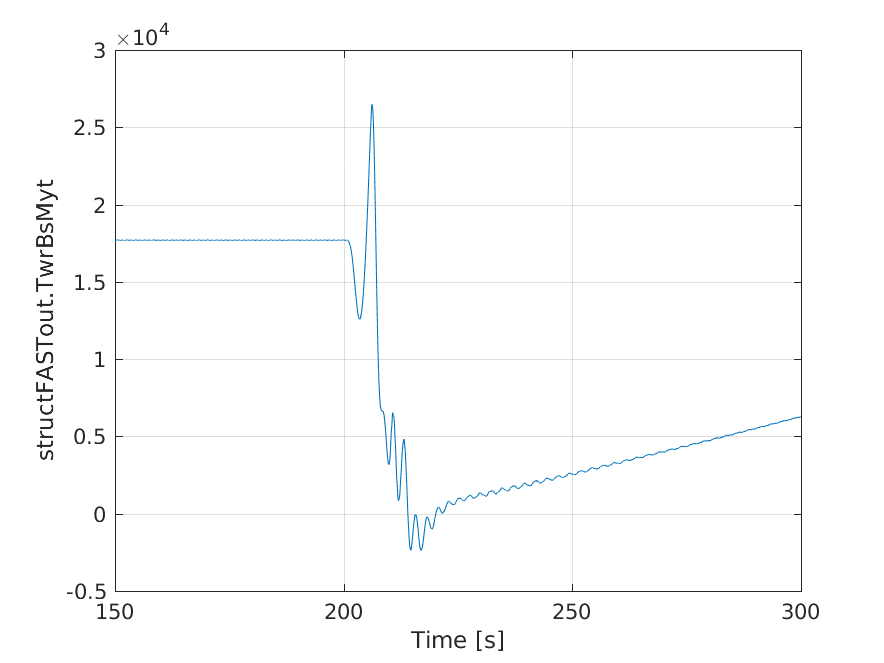
\includegraphics[width=1\linewidth]{../CIP_6/FASTextreme/EOG_50/TwrBsMyt.png}
    \caption{Tower fore-aft for EOG\_50}
\end{subfigure}
\begin{subfigure}{0.40\textwidth}
  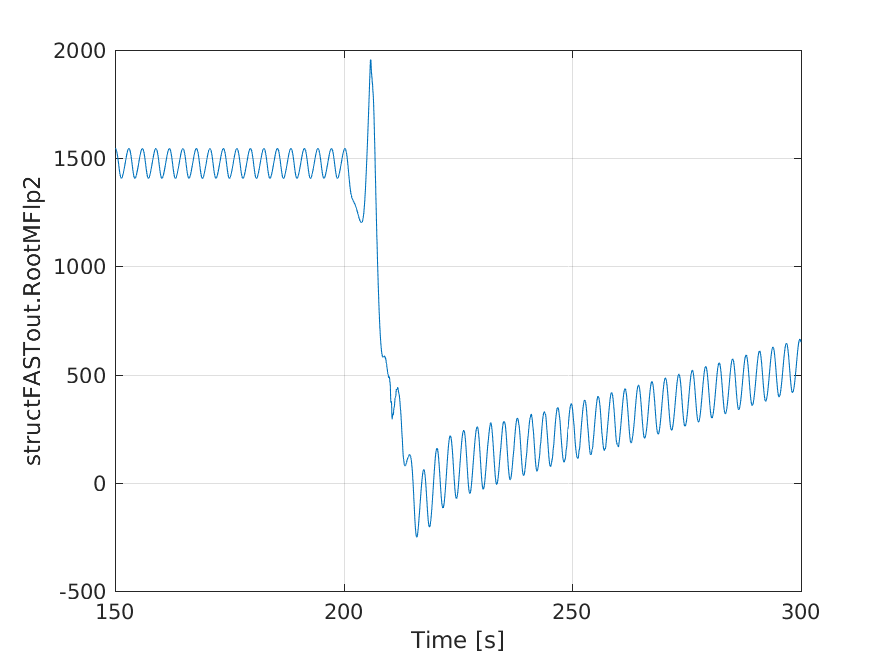
\includegraphics[width=1\linewidth]{../CIP_6/FASTextreme/EOG_50/RootMFlp2.png}
    \caption{Blade flapwise for EOG\_50}
\end{subfigure}
\caption{Time series EOG}
\label{fig:lc23signal}
\end{figure}

Let us have a look at the time series now. For load case 2.3 we consider the same sensors as in the fatigue analysis (tower fore-aft and blade flapwise bending moments) for the 50-year return gust, see Figure~\ref{fig:lc23signal}. With the occurrence of the gust and the failure a high peak in both signals follows and after that a steep decrease to zero with some oscillations and then a slow recovering of the signal. The reaction of the controller accounts for this behavior, because it changes the pitch angle in order to cope with the gust, see Figure~\ref{fig:lc23pitch}.
\begin{figure}[H]
  \centering
  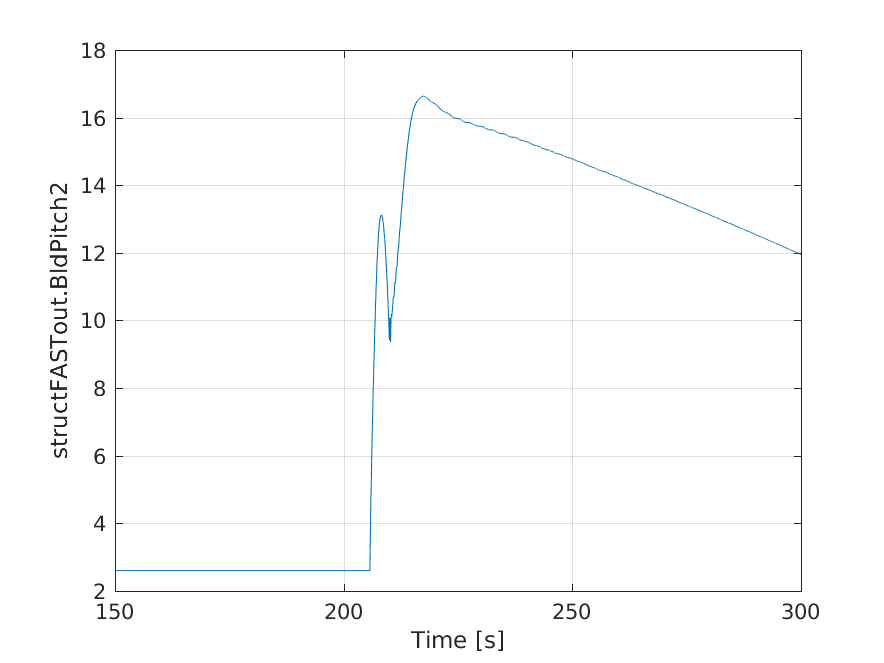
\includegraphics[width=0.4\linewidth]{../CIP_6/FASTextreme/EOG_50/BldPitch2.png}
    \caption{Pitch for EOG\_50}
\label{fig:lc23pitch}
\end{figure}

The signals for the 1-year return gust look similar (here a gust of +4.5m/s is simulated instead of +6m/s as in the case of the 50-year gust).\\
For load case 1.5 we obtain the signals in Figure~\ref{fig:lc15signal}.

\begin{figure}[H]
  \centering
\begin{subfigure}{0.40\textwidth}
  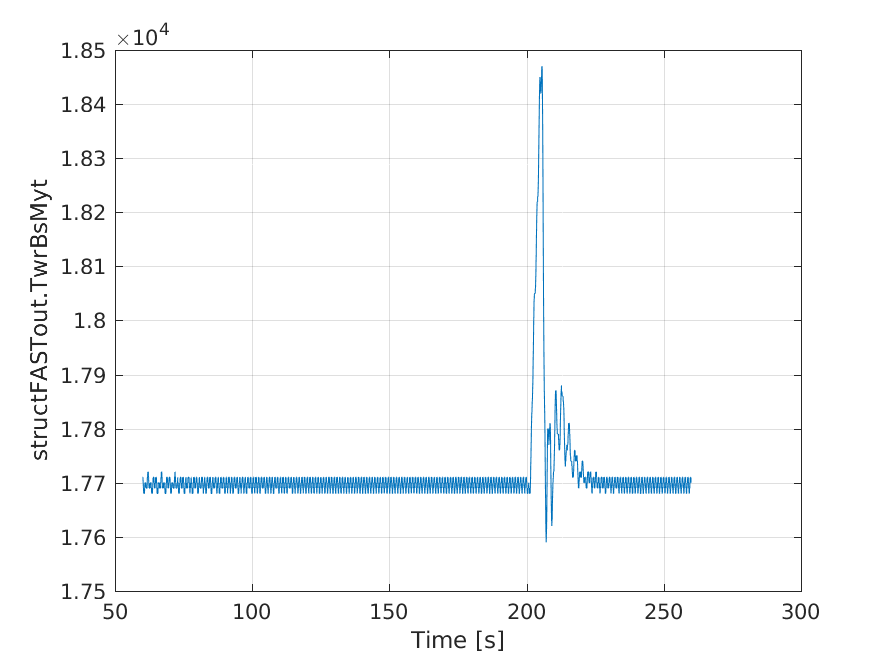
\includegraphics[width=1\linewidth]{../CIP_6/FASTextreme/EWSVR/TwrBsMyt.png}
    \caption{Tower fore-aft for EWS}
\end{subfigure}
\begin{subfigure}{0.40\textwidth}
  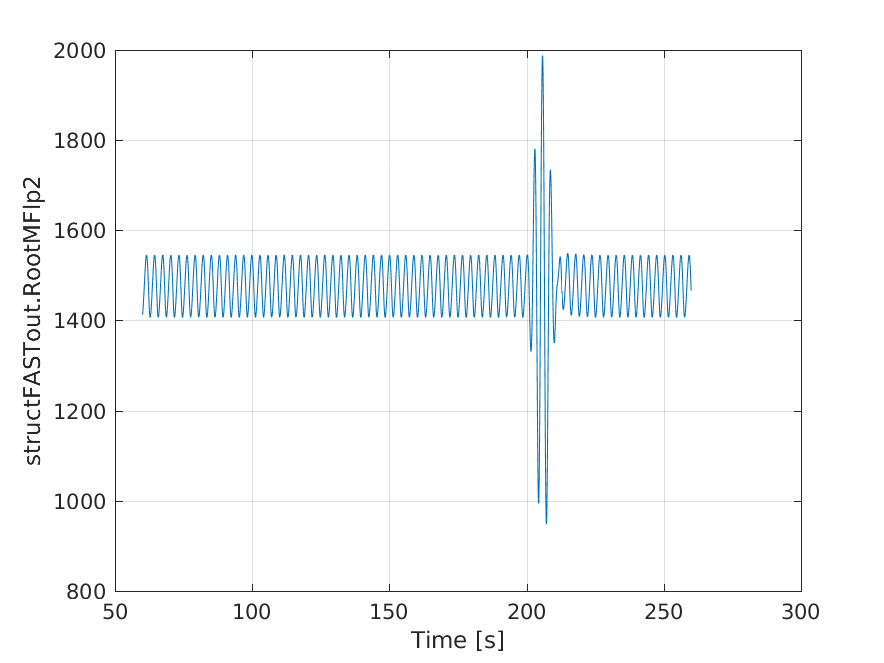
\includegraphics[width=1\linewidth]{../CIP_6/FASTextreme/EWSVR/RootMFlp2.png}
    \caption{Blade flapwise for EWS}
\end{subfigure}
\caption{Time series EWS}
\label{fig:lc15signal}
\end{figure}

Here we note that the extreme shear event also causes a peak in the signals, which is however especially for the tower not as high as in the case of EOG. Also recovery of the signal is much quicker: After only about 10 seconds the signals have returned to normal oscillations as before the extreme event. Likewise the controller reacted by adapting pitch angles of the blades in order to reduce power and loads due to the extreme shear.\\

No impact could be found regarding the timing of the failure except a shift of the event on the timescale.
Concerning the influence of the brake we modified the input parameters a little. Activation time and time for nominal torque of the brake were considerably reduced (about 25\%) while the nominal torque of the break was increased (around 20\%).
The recovery of the signal now goes much faster, see Figure~\ref{fig:lc23breaksignal}. Here the signal already drops back to the values before the event at around $t=300s$ whereas with the original brake settings this process takes approximately twice as long (compare Figure~\ref{fig:lc23signal}.

\begin{figure}[H]
  \centering
\begin{subfigure}{0.40\textwidth}
  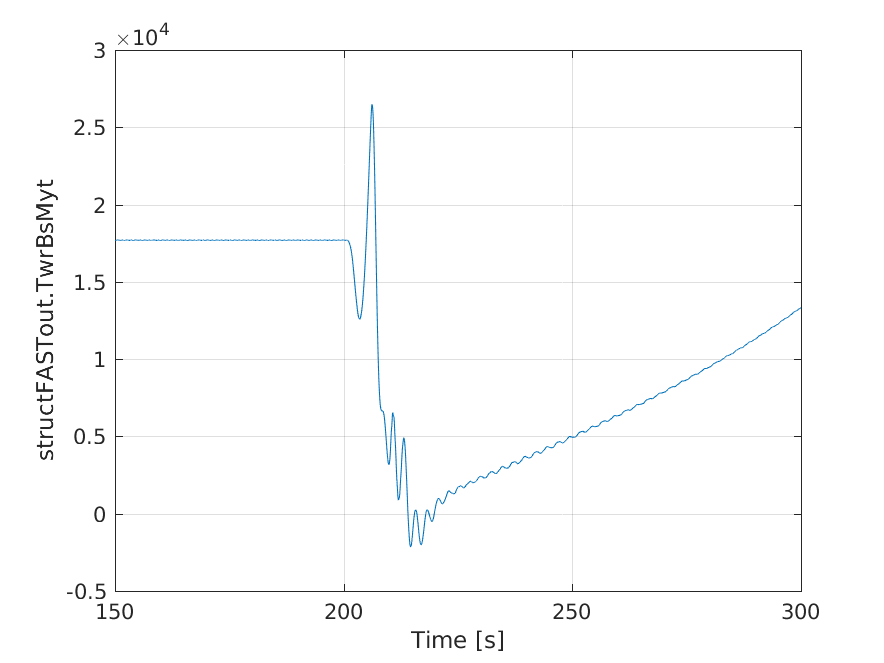
\includegraphics[width=1\linewidth]{../CIP_6/FASTextreme/EOG_50_brake/TwrBsMyt.png}
    \caption{Tower fore-aft}
\end{subfigure}
\begin{subfigure}{0.40\textwidth}
  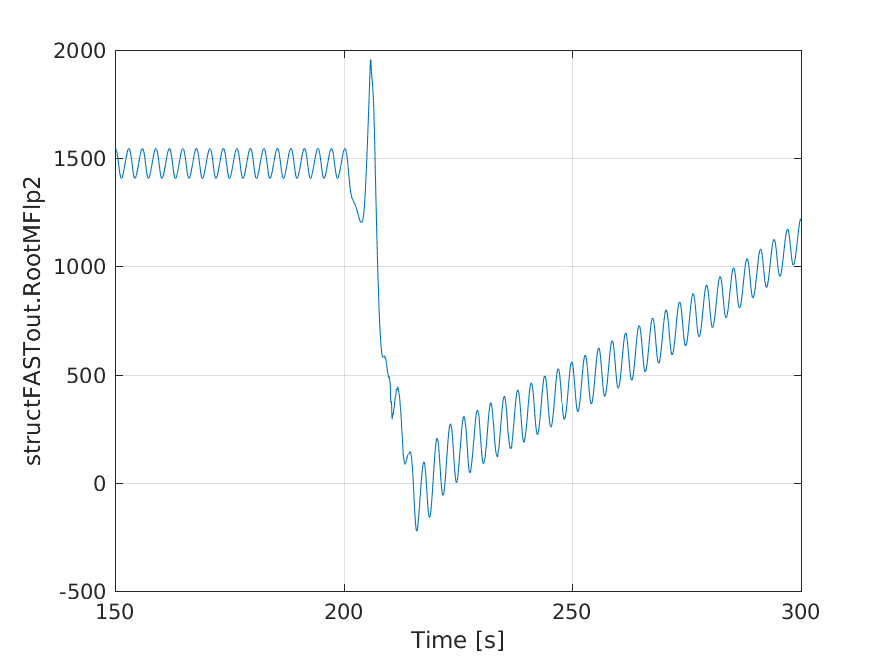
\includegraphics[width=1\linewidth]{../CIP_6/FASTextreme/EOG_50_brake/RootMFlp2.png}
    \caption{Blade flapwise}
\end{subfigure}
\caption{Modified breaks for EOG\_50}
\label{fig:lc23breaksignal}
\end{figure}

A change in the time of the failure (TimeGenOf in the input file) does also affect the signal. We have had the failure occur before the extreme gust. The corresponding signal can be found in Figure~\ref{fig:lc23failtime}.
After the failure the signal drops to zero and then the gust appears and the return to normal operation of the turbine starts.
\begin{figure}[H]
  \centering
\begin{subfigure}{0.40\textwidth}
  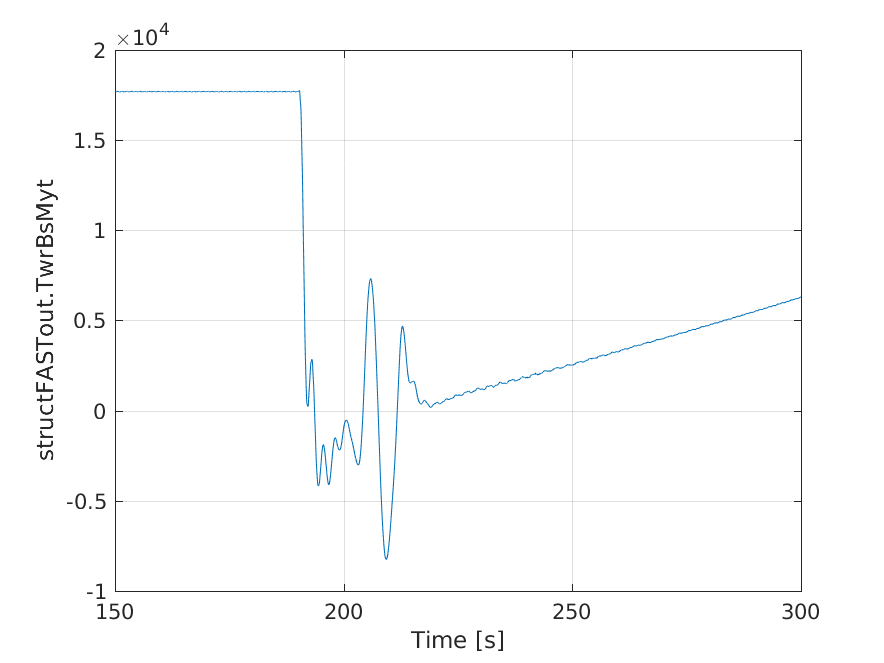
\includegraphics[width=1\linewidth]{../CIP_6/FASTextreme/EOG_50_failtime/TwrBsMyt.png}
    \caption{Tower fore-aft}
\end{subfigure}
\begin{subfigure}{0.40\textwidth}
  \includegraphics[width=1\linewidth]{../CIP_6/FASTextreme/EOG_50_failtime/RootMFlp2.png}
    \caption{Blade flapwise}
\end{subfigure}
\caption{Changed failure time for EOG\_50}
\label{fig:lc23failtime}
\end{figure}


\subsection{Extreme load table}

\begin{table}[H]
\centering
\begin{tabular}{ | l | l | l | l | l | l | }
\hline
	\textbf{Group} & \textbf{Variable} & \textbf{Min/Max} & \textbf{DLC 1.5 EWS} & \textbf{DLC 2.3 EOG01} & \textbf{DLC 2.3 EOG50} \\ \hline \hline
	Tower base & Fx & Min & 206.9 & -36.4 & -20.01 \\ \hline
	Tower base & Fx & Max & 219.5 & 326.5 & 324.8 \\ \hline
	Tower base & Fy & Min & -10.1 & -56.23 & -59.6 \\ \hline
	Tower base & Fy & Max & 1.61 & 49.4 & 47.23 \\ \hline
	Tower base & Fz & Min & -2002 & -2000 & -2001 \\ \hline
	Tower base & Fz & Max & -1993 & -1969 & -1971 \\ \hline
	Tower base & Mx & Min & 630.9 & -1680 & -2084 \\ \hline
	Tower base & Mx & Max & 1630 & 2216 & 2567 \\ \hline
	Tower base & My & Min & 17590 & -3825 & -2380 \\ \hline
	Tower base & My & Max & 18470 & 26580 & 26490 \\ \hline
	Tower base & Mz & Min & -47.01 & -114.7 & -115 \\ \hline
	Tower base & Mz & Max & 158.4 & 65.48 & 67.85 \\ \hline
	Blade root & Fx & Min & 51.93 & -7.054 & -2.584 \\ \hline
	Blade root & Fx & Max & 99.58 & 97.53 & 101.2 \\ \hline
	Blade root & Fy & Min & -53.65 & -53.05 & -53.83 \\ \hline
	Blade root & Fy & Max & 28.19 & 38.35 & 38.11 \\ \hline
	Blade root & Fz & Min & 196.9 & 184 & 186.2 \\ \hline
	Blade root & Fz & Max & 281.2 & 339.1 & 337.6 \\ \hline
	Blade root & Mx & Min & -296.2 & -470.9 & -465.8 \\ \hline
	Blade root & Mx & Max & 726.5 & 684.5 & 710.5 \\ \hline
	Blade root & My & Min & 947.5 & -277.6 & -185.3 \\ \hline
	Blade root & My & Max & 1966 & 1839 & 1943 \\ \hline
	Blade root & Mz & Min & 0.7765 & -0.4313 & -0.4882 \\ \hline
	Blade root & Mz & Max & 12.05 & 16.25 & 13.77 \\ \hline
\end{tabular}
\caption{Extreme load table}
\label{tab:exloadtable}
\end{table}

For tower base and blade root all max and min values of the 6 variables have been extracted from the signal data in Matlab. Values are in KN (forces) and kNm (moments). The first observation is that load case 2.3 dominates load case 1.5 with respect to the amplitudes. The more extreme values of the time series occur in the last and before-last column of the table. Only for some variables we find higher amplitudes for load case 1.5, e.g. TwrBsFzt and TwrBsMzt. 
Within the load case 2.3 there is no clearly dominant setting. The 1-year gust and the 50-year gust setting both have similar amplitudes in the signals. Sometimes EOG\_01 has lower min or higher max values and sometimes EOG\_50 wins.

\section{Summary}
In this design project the entire process of designing a wind turbine has been carried out. We have seen that it is a very complex undertaking requiring a lot of expertise from engineering, physics and also meteorology. The team has to be very accurate at any point and take into account a lot of aspects. The site conditions must be investigated in order to find out about the possible revenues of the turbine and thus the financial revenue during its lifetime. Economic feasibility is the pre-condition of the whole project for all stakeholders.
The wind distribution, the design of the rotor blade and the mechanical
and electrical efficiency must be taken into account. Wind turbine dynamics are an important aspect as well. Many design decisions must be met which influence the possible energy gain and also the further design process. Security is the next big topic. A load analysis has to be carried out regarding fatigue and extreme loads, otherwise the turbine can not be certified.
All these steps and many more which have not been treated in this project require a professional team and a good time-management in order to successfully design a good turbine.

\end{document}